% % part: 微分方程
% % chap: 偏微分方程
% \documentclass[UTF8]{ctexbook}

% \ctexset{
%     part/number = \chinese{part}
% }
% \usepackage{multirow}
% \usepackage{amsmath}% ams 数学公式
% \usepackage{mathtools}% ams 数学公式
% \usepackage{amsfonts}% ams 数学字体
% \usepackage{amssymb,latexsym}% ams 数学符号与LaTeX数学符号
% \usepackage{mathrsfs}% 花式符号
% \usepackage{ntheorem}%定理、定义、证明
%   \theoremstyle{nonumberplain}
%   \theoremheaderfont{\bfseries}
%   \theorembodyfont{\normalfont}
%   \theoremsymbol{$\square$}
%   \newtheorem{Proof}{\hskip 2em 证明}
%   \newtheorem{theorem}{\hspace{2em}定理}[chapter]
%   \newtheorem{definition}{\hspace{2em}定义}[chapter] % 如果没有章, 只有节, 把上面的[chapter]改成[section]
%   \newtheorem{axiom}[definition]{\hspace{2em}公理}
%   \newtheorem{lemma}[definition]{\hspace{2em}引理}
%   \newtheorem{proposition}[definition]{\hspace{2em}命题}
%   \newtheorem{corollary}[definition]{\hspace{2em}推论}
%   \newtheorem{remark}{\hspace{2em}注}[chapter] %类似地定义其他“题头”. 这里“注”的编号与定义、定理等是分开的
% %算法伪代码
% %http://blog.csdn.net/lwb102063/article/details/53046265
% \usepackage{algorithm}
% \usepackage{algorithmicx}
% \usepackage{algpseudocode}
%     \floatname{algorithm}{算法}
%     \renewcommand{\algorithmicrequire}{\textbf{输入:}}
%     \renewcommand{\algorithmicensure}{\textbf{输出:}}

% \usepackage{enumerate}%itemiz环境。\begin{enumerate}[step 1][a)]可以使用 A,a,I,i,1 作为可选项产生
% \usepackage{cite}%参考文献
%     \bibliographystyle{plain}
% \usepackage{extarrows}% 带参数的箭头
% \usepackage{hyperref}% 超链接
% %\usepackage[CJKbookmarks, colorlinks, bookmarksnumbered=true,pdfstartview=FitH,linkcolor=black,citecolor=black]{hyperref}%超链接的格式设置
% \hypersetup{
%     colorlinks=false,% 去掉超链接颜色
%     pdfborder=0 0 0% 取消超链接的边框
% }
% \usepackage{graphicx}% 图片管理
% \usepackage{caption}
% \usepackage{subcaption}%并排的图各有标题
% \graphicspath{{images/}}% 设置图片搜索路径
% \usepackage{float,varwidth}% 浮动体
% \usepackage{booktabs}% 三线表
% \usepackage{fancyhdr}% 页眉设置
% \usepackage{xcolor}% 颜色宏包
% \usepackage{colortbl}% 彩色表格
% \usepackage{listings}% 代码高亮
% \usepackage{caption}% 对标题进行控制,如让\caption标题的字体缩小一号,同时数字标签使用粗体可以用:\usepackage[font=small,labelfont=bf]{caption}
% \usepackage{xfrac,upgreek}%分别是行间公式如a/b的形式(将原来的命令\frac改成\sfrac)和希腊字体的宏包的
% \usepackage{mathtools}%lgathered和rgathered环境把公式向左向右对齐
% \usepackage{tabularx}%提供自动延伸的表列,(X列格式说明符),文字过长时可以自动转行
% \usepackage{longtable}%长表格
% \usepackage{enumitem}%enumerate宏包的升级
% \usepackage{harpoon}%数学公式的矢量
% \usepackage{bookmark}%目录的书签
% \usepackage{pifont}%给数字加上圈。然后在正文输入\ding{172}~\ding{211}得到相应数字,要是要①就输入:\ding{172}②就输:\ding{173}
% \renewcommand{\headwidth}{\textwidth}%图片并排,这个要列在所有宏包的后面
% \makeatletter
% \newcommand{\rmnum}[1]{\romannumeral #1}
% \newcommand{\Rmnum}[1]{\expandafter\@slowromancap\romannumeral #1@}
% \makeatother%这4行是使用罗马数字,然后在正文中使用命令\rmnum{数字},Rmnum{数字}来分别显示大小写罗马数字
% \definecolor{codegreen}{rgb}{0,0.6,0}
% \definecolor{codegray}{rgb}{0.5,0.5,0.5}
% \definecolor{codepurple}{rgb}{0.58,0,0.82}
% \definecolor{backcolour}{rgb}{0.95,0.95,0.92}
% \lstset{
%     commentstyle=\color{codegreen},
%     keywordstyle=\color{magenta},
%     numberstyle=\tiny\color{codegray},
%     stringstyle=\color{codepurple},
%     basicstyle=\footnotesize,
%     breakatwhitespace=false,% 断行只在空格处
%     breaklines=true,% 自动断行
%     captionpos=b,% 标题位置
%     keepspaces=true,
%     numbers=left,
%     numbersep=5pt,
%     showspaces=false,
%     showstringspaces=false,
%     showtabs=false,% 显示
%     tabsize=2% TAB 被当作两个空格
% }
% \topmargin=0pt\oddsidemargin=0pt\evensidemargin=0pt
% \textwidth=16.5cm\textheight=23cm\raggedbottom%我这么设置是为了缩小页边距,满足有的文字无法转行
% \pagestyle{headings}%页眉为章节标题,无页脚
% \setlength{\abovecaptionskip}{4pt}
% \setlength{\belowcaptionskip}{-8pt}%图片表格的前后距离设置
% \CTEXsetup[format={\zihao{-3}\raggedright\bfseries}]{section}%设置节的格式


% \begin{document}
% \part{微分方程}
	% \label{prt:de}
\chapter{偏微分方程}
	% \label{cha:pde}
% \chapter{积分方程}
% \chapter{随机微分方程}
% \chapter{倒向随机微分方程}
\section{偏微分方程建模}
    \subsection{热传导方程}
        我们仅研究均匀介质的固体热传导问题,如果是关于液体和气体的热传导,则需要重新推导热传导方程的形式。下面,我们考虑这样一个问题:对一物体(固)进行加热,问不同时间$t$时,物体各部分的温度是多少?
        \par
        可以想象,在物体内的一点产生初始热量(最初物体温度均匀),热量向各个方向$(x,y,z)$扩散应该是一致的。不妨将问题简化到一维情况,比如仅考虑$x$方向上的。考虑一个极细杆(一维)的热传导过程,如图(\ref{fig:一维热传导示意图})所示\\
		 \begin{figure}[H]
		\centering
		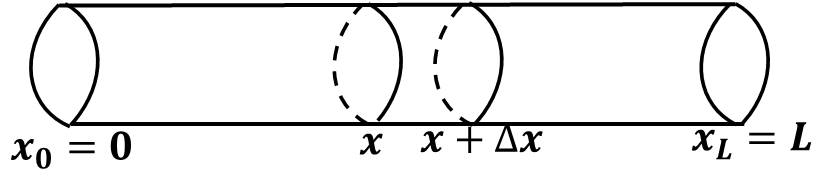
\includegraphics[width=6cm]{images/One_dimensional_heat_conduction.jpg}
		\caption{一维热传导示意图}
		\label{fig:一维热传导示意图}
		\end{figure}
        \par
        设杆的横截面积为$A$,杆的长度为$L$,假设同介质且密度均匀,密度为$\rho$。我们用$u(x,t)$表示$t$时刻$x$点处的温度,用$e(x,t)$表示热能密度,即单位体积上的热能,则$[x,x+\Delta x]$内具有的热能为$e(x,t) A \Delta x$。
        \par
        考虑$[x,x+\Delta x]$段内热能的瞬时变化率,由热量守恒,我们知道热能的瞬时变化是瞬时从$x$面内进入的能量减去瞬时从$x + \Delta x$面内出去的热量,再加上瞬时内部($[x,x+\Delta x]$段自身)产生的热量,有
        \begin{align}
            \label{热能瞬时变化率}
            \frac{\partial}{\partial t} e(x,t)A \Delta x \approx \phi(x,t)A - \phi (x+\Delta x, t) A + Q(x,t) A \Delta x
        \end{align}
        其中:$\phi(x,t)$为热通量,表示单位时间(瞬时)通过$x$处的热量;$Q(x,t)$为热源,表示单位时间物体自身所产生的热量。
        \par
        将上式(\ref{热能瞬时变化率})两边同除$\Delta x$,并令$\Delta x\rightarrow 0$,有
        \begin{align*}
            \frac{\partial e}{\partial t} &= \lim_{\Delta x \rightarrow 0} \frac{\phi (x,t) - \phi (x + \Delta x,t)}{\Delta x} + Q(x, t) \\
            &= \frac{\partial \phi }{\partial x} + Q
        \end{align*}
        下面,我们来讨论$e(x,t)$和$\phi(x,t)$。
        $e(x,t)$为热能密度,其和温度$u(x, t)$的关系为
        \[
            e(x,t) = c(x)\rho (x) u(x,t)
        \]
        其中:$c(x)$为物体比热容,$\rho(x)$为物体密度。
        \par
        $\phi (x, t)$表示单位时间(瞬时)进入的热量,它和温度$u(x,t)$有关,两侧温差越大,热能流动速度越快,热能由高温物体流向低温物体。由傅里叶热传导定律,我们有
        \[
            \phi (x,t) = -k_0\frac{\partial u}{\partial x}
        \]
        其中:$k_0$为导热系数,与物体的材料有关;$\frac{\partial u}{\partial x}$可以表示单位温差,与$\phi$成比例。
        \par
        整理方程,得到
        \begin{align}
            \label{一维扩散方程}
            c \rho \frac{\partial u}{\partial t} &= \frac{\partial}{\partial x}(k_0 \frac{\partial u}{\partial x}) + Q \notag\\
            &= k_0\left( \frac{\partial^2 u}{\partial x^2} \right) + Q
        \end{align}
        我们将$Q$视为恒定热源,$c,\rho , k_0$皆与物体有关,是物体的属性,在给定具体的物体后,不妨将其视为常量(均匀分布)。上述方程(\ref{一维扩散方程})描述了热能是如何展开(扩散),是一个通用的扩散过程,如化学污染物,大气污染物等等的扩散,皆可描述为上述扩散过程(\ref{一维扩散方程}),因此,方程(\ref{一维扩散方程})也被成为扩散方程。
        \par
        由于各个方向$(x,y,z)$的相似性,我们很容易将上述方程(\ref{一维扩散方程})扩展到三维空间
        \begin{align}
            \label{三维扩散方程}
            c \rho \frac{\partial u}{\partial t} = k_0\left( \frac{\partial^2 u}{\partial x^2} + \frac{\partial^2 u}{\partial y^2} + \frac{\partial^2 u}{\partial z^2}\right ) + Q
        \end{align}
        不妨记
        \begin{align*}
            \triangle u = \nabla^2 u = \frac{\partial^2 u}{\partial x^2} + \frac{\partial^2 u}{\partial y^2} + \frac{\partial^2 u}{\partial z^2}
        \end{align*}
        称$\nabla^2 u $为$u$的双哈密顿算子形式,$\triangle u$为$u$的拉普拉斯算子形式。
        于是上式(\ref{三维扩散方程})写为算子形式有
        \begin{align*}
            c \rho \frac{\partial u}{\partial t} = k_0 \nabla^2 u + Q
        \end{align*}
        \par
        我们定义热传导方程(\ref{三维扩散方程})的稳态:当温度$u(x,t)$不再随时间而改变,即
        \[
            \frac{\partial u}{\partial t} = 0
        \]
        此时的状态为稳态。于是,我们有
        \begin{align}
            \label{泊松方程}
            \nabla^2 u = - \frac{Q}{k_0}
        \end{align}
        称上述方程(\ref{泊松方程})为泊松方程。$\nabla^2 u = 0$为拉普拉斯方程(拉普拉斯算子$\nabla^2$的方程)。
        \par
        上面的热传导方程(\ref{三维扩散方程})比较适用于物体形状是长方体的情况,当物体是圆柱或者球体时,可以进行相应的坐标变换,例如:对$x,y,z$进行柱面坐标变换,令
        \begin{align*}
            \left\{
                \begin{aligned}
                    &x = r\cos\theta\\
                    &y = r\sin\theta\\
                    &z = z
                \end{aligned}
            \right.
        \end{align*}
        有
        \[
            \nabla^2 u = \frac{1}{r} \frac{\partial}{\partial r}\left( r \frac{\partial u}{\partial r}\right) +
            \frac{1}{r^2}\frac{\partial^2 u}{\partial \theta ^2} + \frac{\partial^2 u}{\partial z^2}
        \]
        对$x,y,z$进行球面坐标变换,令
        \begin{align*}
            \left\{
                \begin{aligned}
                    &x = \rho\sin \phi\cos\theta\\
                    &y = \rho\sin \phi\sin\theta\\
                    &z = \rho\cos \phi
                \end{aligned}
            \right.
        \end{align*}
        有
        \[
            \nabla^2 u = \frac{1}{\rho^2} \frac{\partial}{\partial \rho } \left( \rho^2 \frac{\partial u}{\partial \rho}\right) +
            \frac{1}{\rho^2 \sin \phi} \frac{\partial}{\partial \phi }\left( \sin \phi\frac{\partial u}{\partial \phi}\right) +
            \frac{1}{\rho^2 \sin ^2\phi} \frac{\partial^2 u}{\partial \theta ^2}
        \]

    \subsection{弦振动方程}
        \label{sub:弦振动方程}
        \par
        考虑柔软均匀的细弦,将弦两端固定,当受到与平衡位置垂直的外作用力时,弦开始振动。假设运动发生在同一平面(仅上下振动),求不同时间$t$弦上各点的坐标,也就是求不同时间$t$的弦曲线。\\
        \ding{172}建系
        \par
        以弦左端点处为坐标原点$O$点,以弦平衡(静止)位置为$x$轴,垂直向上为$u$轴,建立坐标系$xOu$,如图(\ref{fig:弦振动示意图})所示
		\begin{figure}[H]
    		\centering
    		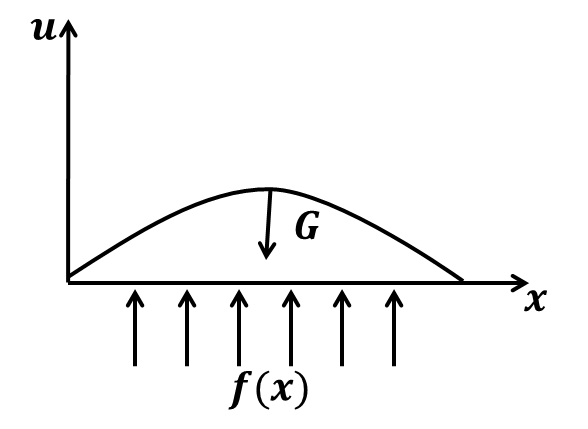
\includegraphics[width=5cm]{images/string_vibration.jpg}
    		\caption{弦振动示意图}
    		\label{fig:弦振动示意图}
		\end{figure}
        \noindent{\ding{173}定量}
        \par
        设弦长为$l$,外力为$f(x)$,重力为$G$,求$t$时刻各点位置,即$u(x,t)$,(可以尝试忽略$G$)。\\
        \ding{174}微元法进行受力分析
        \par
        在微元段$[x,x+\Delta x]$上进行受力分析,微元段长度为$\Delta S \approx \Delta x$(当$\Delta x \rightarrow 0$时),弦受重力、外力和张力的作用,其受力分析如图(\ref{fig:弦受力分析示意图})所示
		\begin{figure}[H]
		\centering
		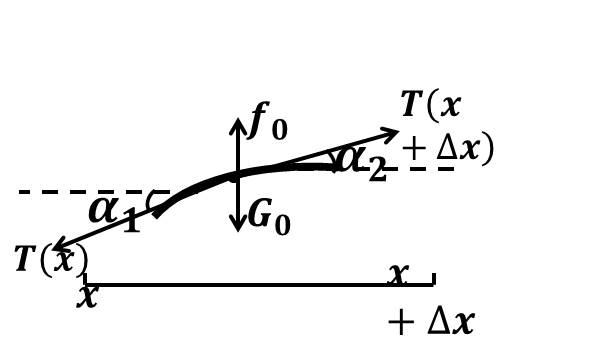
\includegraphics[width=5cm]{images/string_force_analysis.jpg}
		\caption{弦受力分析示意图}
		\label{fig:弦受力分析示意图}
		\end{figure}
        % \textcolor[rgb]{1.00,0.00,0.00}{todo:图片:弦受力分析示意图}\\
        由于弦很柔软,所以张力$T$是沿切线方向的,并且由胡克定律可知,$T$与时间$t$无关,否则要写成$T(x,t)$。由短时间内受力平衡,我们有
        \begin{align}
            \label{弦受力平衡方程}
            \left\{
                \begin{aligned}
                    &T(x+\Delta x_0) \cos \alpha _2 = T(x) \cos \alpha_1\\
                    &T(x+\Delta x_0) \sin \alpha _2 + f_0 \Delta x = T(x) \sin \alpha_1 +G_0 +\rho \Delta x
                    \frac{\partial ^2 u}{\partial t^2} \notag
                \end{aligned}
            \right.
        \end{align}
        其中:$\rho$为单位弦长的密度;$\frac{\partial ^2 u}{\partial t^2}$表示$u$方向上的加速度,$f_0(x,t)$为力$F$单位长度的力。
        \par
        在$\Delta x \rightarrow 0$时,有$G_0 \rightarrow 0$,并且有$\cos \alpha _1 \approx \cos \alpha _2 \approx 1$,以及
        \begin{align*}
            &\sin \alpha_1 \approx \tan \alpha_1 = \frac{\partial u(x,t)}{\partial x}\\
            &\sin \alpha_2 \approx \tan \alpha_2 = \frac{\partial u(x + \Delta x,t)}{\partial x}
        \end{align*}
        我们可以假定$T(x) \approx T(\Delta x + x) = T_0$,即张力$T$为常量,将其带入到(\ref{弦受力平衡方程})方程当中,有
        \begin{align}
            %\label{弦振动方程1}
            \rho \Delta x \frac{\partial^2 u}{\partial t ^2} \approx T_0 \left ( \frac{\partial u(x + \Delta x,t)}{\partial x} - \frac{\partial u(x,t)}{\partial x} \right) + f_0\Delta x
        \end{align}
        将上式两边同除$\Delta x$,并且令$\Delta x \rightarrow 0$,有
        \begin{align}
            \label{弦振动方程2}
            \rho \frac{\partial^2 u}{\partial t ^2} = T_0 \frac{\partial^2 u}{\partial x^2} + f_0
        \end{align}
        由弦均匀,我们知道密度$\rho$为常数,记
        \[
            \frac{T_0}{\rho} = a^2,\quad \frac{f_0}{\rho} = f(x,t)
        \]
        带入式(\ref{弦振动方程2}),整理后有
        \begin{align}
            \label{弦振动方程3}
            \rho \frac{\partial^2 u}{\partial t ^2} = a^2 \frac{\partial^2 u}{\partial x^2} + f(x,t)
        \end{align}
        上式(\ref{弦振动方程3})即为弦振动的一般方程。

    \subsection{膜振动方程}
        \par
        我们应该在二维情况下考虑薄膜的振动,三维情况下考虑“体”的振动。这里,我们仅对振动的一维情况(\ref{弦振动方程2})做一个简单的推广:在二维情况下,有薄膜振动方程
        \begin{align}
            \label{薄膜振动方程}
            \rho \frac{\partial^2 u}{\partial t ^2} = T_0\left ( \frac{\partial^2 u}{\partial x^2} + \frac{\partial^2 u}{\partial y^2} \right )+ f(x,y,t)
        \end{align}
        在三维情况下(声波、电磁波等在空间中的传播),有如下振动方程
        \begin{align}
            \label{声波振动方程}
            \frac{\partial^2 u}{\partial t ^2} = a^2 \left ( \frac{\partial^2 u}{\partial x^2} + \frac{\partial^2 u}{\partial y^2} + \frac{\partial^2 u}{\partial z^2} \right )+ f(x,y,z,t)
        \end{align}

\section{偏微分方程基本理论}
    \subsection{三大基本方程}
    \par
    在介绍经典偏微分的三大方程之间,我们先来介绍一下哈密顿算子和拉普拉斯算子:定义哈密顿算子$\nabla$为
    \[
        \nabla = i\frac{\partial}{\partial x} + j\frac{\partial}{\partial y} + k\frac{\partial}{\partial z} = grid
    \]
    其中:$i,j,k$是$x,y,z$方向上的单位向量,哈密顿算子是具有方向的算子。
    \par
    定义拉普拉斯算子$\triangle$为
    \[
        \triangle = \frac{\partial}{\partial x^2} + \frac{\partial}{\partial y^2} + \frac{\partial}{\partial z^2}
    \]
    拉普拉斯算子是不具有方向的标量算子,并且有
    \[
        \triangle = \nabla \nabla = \nabla^2
    \]
    \par
    下面,来介绍经典偏微分的三大基本方程:波动方程(双曲型方程)、扩散方程(抛物型方程)和稳态方程(椭圆型方程)。
    \paragraph{波动方程}
    前面引入的弦振动和膜振动等方程即为波动方程,波动方程的特点是方程中含有未知量$u$(待求函数)关于时间$t$的二阶偏导数,一般形式为
    \begin{align*}
        %\label{波动方程一般形式}
        \frac{\partial^2 u}{\partial t ^2} = a^2 \left ( \frac{\partial^2 u}{\partial x^2} + \frac{\partial^2 u}{\partial y^2} + \frac{\partial^2 u}{\partial z^2} \right )+ f(x,y,z,t)
    \end{align*}
    此方程用于描述弦、膜、波、传输线上电流电压等物理量的变化规律。可以看出,由于$u$是时变的,所以,求解得到的$u$是一个随时间$t$变化而变化的三维立体(曲面)$u(x,y,z,t)$,即是一个动图。
    \paragraph{扩散方程}
    前面引入的热传导方程即为扩散方程,扩散方程的特点是方程中含有$u$对时间$t$的一阶偏导,其一般形式为
    \begin{align*}
        %\label{扩散方程一般形式}
        \frac{\partial u}{\partial t} = a^2 \left ( \frac{\partial^2 u}{\partial x^2} + \frac{\partial^2 u}{\partial y^2} + \frac{\partial^2 u}{\partial z^2} \right )+ f(x,y,z,t)
    \end{align*}
    此方程用于描述热量扩散、液体渗透、气体和半导体中杂质的扩散过程。
    \paragraph{稳态方程}
    未知函数$u$不随时间$t$变化而变化,即对$\forall n = 1,2,\dots, $,有
    \[
        \left ( \frac{\partial u}{\partial t}\right )^n = 0
    \]
    稳态方程的典型代表是泊松方程和拉普拉斯方程
    \begin{align*}
        & 0 = \frac{\partial^2 u}{\partial x^2} + \frac{\partial^2 u}{\partial y^2} + \frac{\partial^2 u}{\partial z^2} + f(x,y,z)\\
        & 0 = \frac{\partial^2 u}{\partial x^2} + \frac{\partial^2 u}{\partial y^2} + \frac{\partial^2 u}{\partial z^2}
    \end{align*}
    可以看出,这里的$u$不是时变的,与时间$t$无关,所以解为一固定的三维曲面。


    \subsection{偏微分基本定义}
        \par
        1.偏微分方程的一般形式为
        \begin{align}
            \label{偏微分方程的一般形式}
            F\left ( \mathbf{x},\frac{\partial u}{\partial x_1},\dots,\frac{\partial u}{\partial x_n}, \dots,\frac{\partial ^m u}{\partial x_1^{m_1} \partial x_2^{m_2},\dots,\partial x_n^{m_n}}\right) = 0
        \end{align}
        其中:$\mathbf{x} = (x_1,x_2,\dots,x_n)$为自变量,$u$为未知函数,$F$为已知的函数形式,$\sum m_i = m$。
        \par
        2.偏微分方程的阶数。方程中最高阶偏导数的阶即为方程的阶,对上述方程(\ref{偏微分方程的一般形式}),其阶数为$m$。
        \par
        3.显隐性。偏微分方程的显隐性由方程的主函数$F$决定,如果$F$为显函数,则偏微分方程也为显式方程。
        \par
        4.方程的线性与非线性:
        \[
            a \frac{\partial^2 u}{\partial x^2} +b\frac{\partial u}{\partial x} + cu = f(x,t)
        \]
        为线性偏微分方程
        \[
            a \sin \left( \frac{\partial^2 u}{\partial x^2}\right ) +b \cos \left(\frac{\partial u}{\partial x}\right ) + cu = 0
        \]
        为非线性偏微分方程。\par
        5.常系数方程和变系数方程。如果方程的系数是常量,则称为常系数微分方程
        \[
            a \frac{\partial^2 u}{\partial x^2} +b\frac{\partial u}{\partial x} + cu = f(x,t)
        \]
        为常系数方程
        \[
            a(x,y,t) \frac{\partial^2 u}{\partial x^2} +b(x,t)\frac{\partial u}{\partial x} + c(t)u = f(x,t)
        \]
        为变系数方程。\par
        6.齐次与非齐次方程。
        \[
            a \frac{\partial^2 u}{\partial x^2} +b\frac{\partial u}{\partial x} + cu = f(x,t)
        \]
        为非齐次方程
        \[
            a \frac{\partial^2 u}{\partial x^2} +b\frac{\partial u}{\partial x} + cu = 0
        \]
        为齐次方程。

        \subsubsection{7.边值条件}
            \paragraph{初值条件}
            像常微分方程有初值条件和边值条件那样,偏微分方程也有相应的条件。比如,我们可以要求偏微分方程的初始状态为某一具体的函数(曲面)形式。不失为一般性,考虑二维平面$xOy$,在区域$\Omega \in R^2$上求一个函数$u(x,y,t)$,这个函数$u$是时变的,要求这个函数在初始时刻$t_0$的状态为$\varphi (x,y)$,即
            \[
                u(x,y,t) \bigl|_{t=t_0} = u(x,y,t_0) = \varphi (x,y)
            \]
            \par
            上面介绍的是偏微分方程的初值条件,可以想象,求一个时变的曲面$u$,要求其在初始时刻$t_0$的曲面形状就为$\varphi (x,y)$。当然,这个条件在微分方程当中是最简单的,实际问题会有许许多多的条件(约束)。下面,我们再介绍两类常见的边值条件:第一边值条件(Dirichlet条件)、第二边值条件(Neumann条件)以及它们的混合。
            \paragraph{第一边值条件}不失为一般性,考虑二维平面$xOy$,在区域$\Omega \in R^2$的边界$\partial \Omega$上,有一个连续函数$g(x,y)$。我们求一个函数$u(x,y,t)$,要求$u(x,y,t)$不仅满足某一偏微分方程,而且在边界$ \partial \Omega$上等于$g(x,y)$。可以想象,在三维空间中一直有一个曲面$u(x,y,t)$,每个时刻$t$这个曲面是不同的,但要求每个时刻$t$它在边界$\partial \Omega$上等于$g(x,y)$,即
            \[
                u(x,y)\bigl|_{\partial \Omega} = g(x,y)
            \]
            \paragraph{第二边值条件}在区域$\Omega \in R^2$的边界$\partial \Omega$上给定一个连续函数,求$u(x,y,t)$,要求$u(x,y,t)$不仅在$\Omega$内满足偏微分方程,而且在$\partial \Omega$上的任意一个沿$\partial \Omega$的外法线方向$\mathbf{n}$的方向导数$\frac{\partial u}{\partial \mathbf{n}}$存在,并且等于$g$在该点的函数值,即
            \[
                \frac{\partial u}{\partial \mathbf{n}} \Bigl|_{\partial \Omega} = g
            \]
            \paragraph{混合边值条件}我们将前面的第一边值条件和第二边值条件混合,可以得到混合边值问题
            \[
                \frac{\partial u}{\partial \mathbf{n}} +b u \bigl|_{\partial \Omega} = g
            \]
    \par
    限于篇幅,关于偏微分方程解的存在唯一性、偏微分方程组、偏微分方程外问题和稳定性这里不做介绍,有兴趣的可以参考相关的偏微分书籍。
    \par
    若PDE在附加条件$\partial \Omega$和求解域$\Omega$的一定要求下,它的解在已知度量的某函数类中存在并且唯一,并且关于附加条件是稳定的,那么就称该定解问题在相应的函数类中为适定的。在偏微分方程的解法上,我们主要介绍PDE的数值解法,而其古典解析方法:傅里叶变换法、拉普拉斯变换法、分离变量法和格林函数法等在一般理论书籍上均由介绍。后面,我们将主要讨论数值方法:有限差分法、变分法、有限元方法(基于变分法)和谱方法(基于变分法)。

    \subsection{解的存在唯一性*}
    \subsection{偏微分方程组*}
    \subsection{偏微分方程外问题*}
    \subsection{偏微分方程稳定性*}

\section{偏微分方程数值方法}
    \subsection{有限差分法}
        \subsubsection{二维泊松方程第一边值条件}
            \par
            由于泊松方程的解是静态的(与时间$t$无关),因此,我们用泊松方程来介绍差分法的思想。差分法的思想与常微分方程中的欧拉法是相似的,考虑如下二维情况下的含第一边值条件的泊松方程
            \begin{align*}
            \left\{
                \begin{aligned}
                    &0 = \frac{\partial^2 u}{\partial x^2} + \frac{\partial^2 u}{\partial y^2} + f(x,y),\quad (x,y)\in \Omega \\
                    &u(x,y)\bigl|_{\partial\Omega} = g(x,y),\quad (x,y)\in \partial\Omega
                \end{aligned}
            \right.
            \end{align*}
            将其写为一般形式
            \begin{align*}
                \left\{
                \begin{aligned}
                    &-\triangle u =-\left( \frac{\partial^2 u}{\partial x^2} + \frac{\partial^2 u}{\partial y^2} \right) = f(x,y)\\
                    &u(x,y)\bigl|_{\partial\Omega} = g(x,y),\quad (x,y)\in \partial\Omega
                \end{aligned}
                \right.
            \end{align*}
            其中:$\Omega $为自变量$x,y$的定义域,$f(x,y)$和$g(x,y)$为已知的函数形式,$u(x,y)$为待求函数,边界$\partial \Omega$为分段光滑的曲线。注:我们有必要讨论函数$f,g,u$的类型(函数类)。
            \par
            我们记$\Gamma = \partial \Omega$,记$Lu = -\triangle u$。这样,我们就可以避免写$-$符号了。
            有限差分法的基本思想是通过对求解区域网格化离散化,然后建立差分方程求解函数$u$的近似值。我们在区域$\Omega$上取两组平行于$x,y$轴的直线,不妨设为等距
            \begin{align*}
                &x:x_i = ih\quad i = 0,\pm1,\pm2,\dots\\
                &y:y_j = jk\quad j = 0,\pm1,\pm2,\dots
            \end{align*}
            其中:$h,k$为步长,有$x_{i+1} - x_i = h$以及$y_{j+1} - y_j = k$。
		\begin{figure}[H]
		\centering
		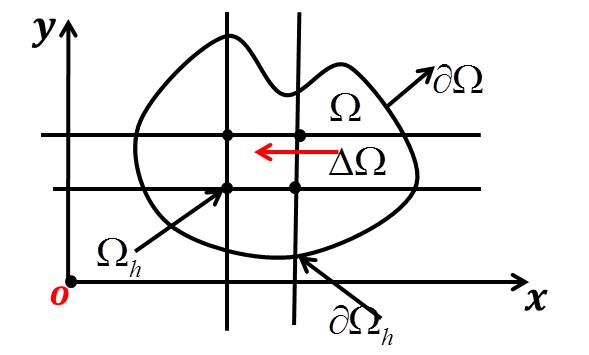
\includegraphics[width=5cm]{images/difference.jpg}
		\caption{差分示意图}
		\label{fig:差分示意图}
		\end{figure}
            % \textcolor[rgb]{1.00,0.00,0.00}{todo:图片:差分示意图}\\
            如图(\ref{fig:差分示意图}),我们设四点所构成的区域为$\Delta \Omega$,$\Omega = \{(x,y)|f\}$。用
            $\Omega_h$表示所有属于$\Omega$网格内的网格点/节点,用$\partial\Omega_h$表示所有位于$\partial\Omega$上的网格点或者节点。
            \par
            为了方便,不妨考虑$\Omega = {(x,y)|a<x<b,c<y<d}$的矩形区域,如图(\ref{fig:矩形差分示意图})所示
		\begin{figure}[H]
		\centering
		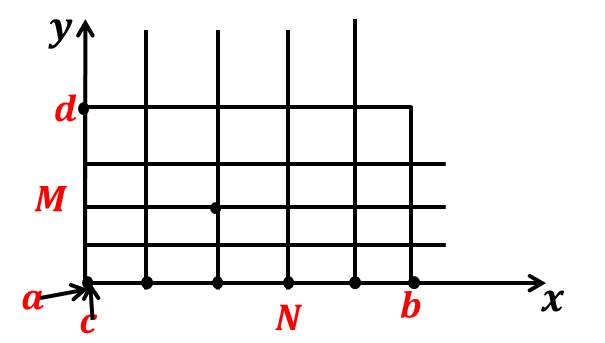
\includegraphics[width=5cm]{images/Rectangular_difference.jpg}
		\caption{矩形差分示意图}
		\label{fig:矩形差分示意图}
		\end{figure}
            % \textcolor[rgb]{1.00,0.00,0.00}{todo:图片:矩形差分示意图}\\
            将$[a,b]$进行$N$等分,将$[c,d]$进行$M$等分,有$h = \frac{b-a}{N},k = \frac{d-c}{M}$,并且,
            \begin{align*}
                &x:x_i = a + ih\quad i = 0,1,\dots, N\\
                &y:y_j = c + jk\quad j = 0,1,\dots, M
            \end{align*}
            两簇指点的交点$(x_i,y_j)$就是网格节点,记为
            \begin{align*}
                &\Omega_h = \left \{ (x_i,y_j)| 0<i<N,0<j<M \right\} \\
                &\partial \Omega_h = \left \{ (x_i,y_j)| i = 0, N,j = 0,1,\dots,M;j = 0,M,i = 0,1,\dots,N \right\}
            \end{align*}
            \par
            边值条件为:在$(x,y) \in \partial \Omega$处有$u = g(x,y)$。像一般的数值解法那样,我们自然希望得到待求函数$u$在各个网格点$(x_i,y_j)$处的函数值$u(x_i,y_j)$,这样就可以用它来估计待求函数$u$。现在的问题是,如果我们知道了$u$在$(x_1,y_1)$处的值$u_1$,如何求$u_2$?一般的,如果我们知道了$(x_i,y_j)$处的函数值$u_{i,j}$,如何求$u_{i+1,j}$处的函数值?
            \par
            像常微分方程那样,我们用差分方程组来进行求解。我们仅就$x$方向来看,已知$u$在$(x_i,y_j)$的函数值$u_i$满足偏微分方程
            \begin{align}
            \label{点的偏微分方程}
                -\triangle u (x_i,y_j) =-\left( \frac{\partial^2 u}{\partial x^2}(x_i,y_j) + \frac{\partial^2 u}{\partial y^2} (x_i,y_j)\right) = f(x_i,y_j)
            \end{align}
            类似
            \[
                f'(x_i) = \frac{f(x_{i+1}) - f(x_i)}{h} - \frac{h}{2} y''(\xi_i)
            \]
            我们将$u$在$(x_{i}\pm h, y_j)$处进行泰勒展开,有
            \begin{align}
                \label{泰勒展开}
               u (x_i\pm h,y_j)
               &= u (x_i h,y_j) \pm h \frac{\partial u}{\partial x}(x_i,y_j) + \frac{h^2}{2} \frac{\partial^2 u}{\partial x^2}(x_i,y_j) \notag\\
               &\quad\pm \frac{h^3}{6} \frac{\partial^3 u}{\partial x^3}(x_i,y_j) + \frac{h^4}{24} \frac{\partial^4 u}{\partial x^4}(\xi_\pm,y_j)
            \end{align}
            其中:$x_i \leqslant \xi_+ \leqslant x_{i+1}$,$x_{i-1} \leqslant \xi_- \leqslant x_{i}$。
            \par
            根据上式(\ref{泰勒展开}),有
            \begin{align}
            \label{x的泰勒展开}
                   &u (x_i + h,y_j) -2u(x_i,y_j) + u(x_i-h,y_j) \notag\\
               ={} &h^2 \frac{\partial^2 u}{\partial x^2}(x_i,y_j) + \frac{h^4}{24} \left[
               \frac{\partial^4 u}{\partial x^4}(\xi_+,y_j) + \frac{\partial^4 u}{\partial x^4}(\xi_-,y_j)
               \right] \notag \\
               ={} &h^2 \frac{\partial^2 u}{\partial x^2}(x_i,y_j) + \frac{h^4}{12} \frac{\partial^4 u}{\partial x^4}(\xi,y_j)
            \end{align}
            其中:$x_{i-1} \leqslant \xi \leqslant x_{i+1}$。
            \par
            在上式的最后一项中,我们利用了和的平均值定理,即如果有$g_i \geqslant 0$且有$\sum _{i =1}^J g_i = 1$,那么$\exists c$,$ \min x_i \leqslant c \leqslant \max x_i$,使得$\sum _{i =1}^J g_if(x_i) = f(c)$成立。类似$x$,我们对$y$也有
            \begin{align}
            \label{y的泰勒展开}
                   &u (x_i ,y_j + k) - 2u(x_i,y_j) + u(x_i,y_j - k) \notag \\
               ={} &k^2 \frac{\partial^2 u}{\partial y^2}(x_i,y_j) + \frac{k^4}{12} \frac{\partial^4 u}{\partial y^4}(x_i,\eta)
            \end{align}
            其中:$y_{j-1} \leqslant \eta \leqslant y_{j+1}$。
            \par
            将式(\ref{x的泰勒展开})除以$h^2$,式(\ref{y的泰勒展开})除以$k^2$,然后将两式相加,可得
            \begin{align}
            \label{u的泰勒展开}
                \Delta u(x_i,y_j) &= \frac{u(x_i+h,y_j) - 2u(x_i,y_j)+u(x_i-h, y_j)}{h^2}\notag \\
                &\quad + \frac{u(x_i,y_j + k) - 2u(x_i,y_j)+u(x_i, y_j - k)}{k^2}\notag \\
                &\quad - \frac{h^4}{12} \frac{\partial^4 u}{\partial x^4}(\xi,y_j) - \frac{h^4}{12} \frac{\partial^4 u}{\partial y^4}(x_i,\eta)
            \end{align}
            上式忽略高阶项$\frac{\partial^4 u}{\partial *^4}$,即可得到$\Delta u(x_i,y_j)$的近似计算公式,然后将$\Delta u(x_i,y_j)$带入(\ref{点的偏微分方程})当中,即可得到如下关系式
            \begin{align}
            \label{5点差分法的等式关系}
                f(x_i,y_j) &= - \frac{u(x_i+h,y_j) - 2u(x_i,y_j)+u(x_i-h, y_j)}{h^2} \notag\\
                &\quad - \frac{u(x_i,y_j + k) - 2u(x_i,y_j)+u(x_i, y_j - k)}{k^2}
            \end{align}
            由此,我们得到了$u(x_i,y_j)$与$u(x_{i+1},y_j)$、$u(x_{i-1},y_j)$、$u(x_i,y_{j+1})$和$u(x_i,y_{j-1})$的等式关系(\ref{5点差分法的等式关系}),其示意图如图(\ref{fig:五点位置示意图})所示,我们称此差分方程为泊松方程的五点差分方程,当然,选用不同阶的泰勒展开公式会得到更多点的差分方程(比如:九点差分方程)。
		\begin{figure}[H]
		\centering
		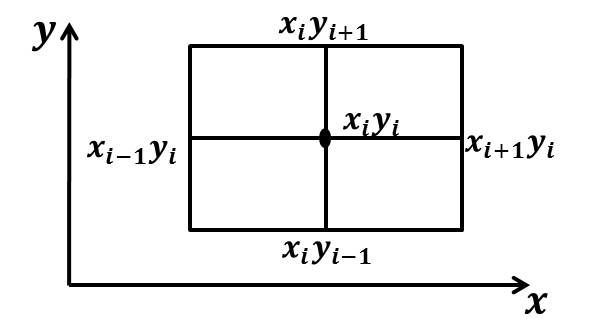
\includegraphics[width=5cm]{images/fivepoint_position.jpg}
		\caption{五点位置示意图}
		\label{fig:五点位置示意图}
		\end{figure}
            % \textcolor[rgb]{1.00,0.00,0.00}{todo:图片:五点位置示意图}
            \par
            综合所有的内点$(x_i,y_j) \in \Omega_h$,我们会得到一个含有$(N-1)\times (M-1)$个未知量$u_{i,j}(i = 1,\dots,N-1,j = 1,\dots,M-1)$(由于边界值已知,所以$i = 0,N$,$y = 0,M$的值已知)的$(N-1)\times (M-1)$阶线性方程组。结合边界点方程
            \[
                u(x_i,y_j) = g(x_i,y_j) \quad (x_i,y_j) \in \partial \Omega_h
            \]
            由此得到$u(x,y)$的数值解。记由线性方程组得到的解为$\hat{u}(x_i,y_j)$,它是$u(x_i,y_j)$的估计。为书写简便,我们将$u(x_i,y_j)$记为$u_{i,j}$,同样有$u_{i+1,j},u_{i-1,j},u_{i,j+1},u_{i,j-1}$,以及它们对应的估计值$\hat{u}_{i,j}$。
            \par
            问一:这种差分方法的数值计算误差哪里来?
            1.步长$h,k$的大小;2.被忽略的高阶项的大小。
            问二:差分方程解的唯一性和收敛性如何?
            \par
            下面,我们讨论(\ref{5点差分法的等式关系})的截断误差。在计算(\ref{5点差分法的等式关系})的时候,我们忽略了(\ref{u的泰勒展开})的高阶项$\frac{\partial^4 u}{\partial *^4}$从而带来误差,令
            \begin{align*}
                \max_{(x,y) \in \Omega} \left| \frac{\partial^4 u}{\partial x^4}(x,y) \right| \leqslant M_4,\quad
                \max_{(x,y) \in \Omega} \left| \frac{\partial^4 u}{\partial y^4}(x,y) \right| \leqslant M_4
            \end{align*}
            则有如下截断误差项的估计
            \begin{align*}
                |R_{i,j}(u)| = \left|  \frac{h^4}{12} \frac{\partial^4 u}{\partial x^4}(\xi,y_j) + \frac{h^4}{12} \frac{\partial^4 u}{\partial y^4}(x_i,\eta) \right| \leqslant \frac{M_4}{12} (h^2+k^2)
            \end{align*}
            所以,五点差分格式的数值计算误差的阶为$|R_{i,j}(u)| = O(h^2+k^2)$。
            \par
            再者,我们讨论差分方法的唯一性和收敛性。这里我们直接给出其收敛性和唯一性定理:
            \begin{theorem}[差分法的收敛性]
            如果泊松方程第一边值问题的解$u(x,y)$在$\Omega \cup \partial \Omega$上有四阶连续偏导数(即$u$是函数类中的一员),则其五点差分的数值解一致收敛到精确解,解唯一并且有
            \[
                \max_{\Omega_h} |\hat{u}_{i,j} - u_{i,j}| \leqslant \frac{C}{12} \max(k,h)^2
            \]
            其中:$C$是与$h,k$无关的常数。
            \end{theorem}

        \subsubsection{二维泊松方程第二边值条件}
            对于Poisson方程的Dirichlet边值问题,前一小节已经详细讨论了其差分格式的建立。可以看出,只需要将边界点处的函数值直接带入差分格式中,就能获得Poisson方程Dirichlet边值问题的有限差分格式。那么对于Neumann边值问题,差分格式的边界条件又如何处理呢?下面具体讨论这一问题,不妨设Poisson方程的第二类边界条件(即Neumann边界条件)为
            \begin{align*}
            \frac{\partial u}{\partial \mathbf{n}} = \alpha ( x,y),\quad ( x,y ) \in \partial \Omega
            \end{align*}
            \par
            为了简单起见,设$\Omega  = \left\{ {\left( {x,y} \right)\left| {0 < x < 1,0 < y < 1} \right.} \right\}$。考虑步长为$h$ 的正方形网格,显然,在正方形的四个顶点上,外法线方向导数$\frac{{\partial u}}{{\partial \mathbf{n}}} $没有定义,这表示$\alpha(x,y)$在顶点处不连续。一般情况下,取平均值来作为不连续点上的函数值。下面讨论Neumann边值问题的有限差分格式,即对$(N+1)^2$个网格点来构造离散的差分格式。
            \par
            首先,对于所有的内节点$(x_i,y_j) \in {\Omega _h}$,由式(\ref{5点差分法的等式关系}),可得离散的差分格式为
            \begin{align}\label{eq:离散差分格式}
             - \frac{1}{{{h^2}}}\left[ {{u_{i + 1,j}} + {u_{i - 1,j}} + {u_{i,j + 1}} + {u_{i,j - 1}} - 4{u_{i,j}}} \right] = {f_{i,j}}\notag\\
             i=1,2,\ldots,N-1; j=1,2,\ldots,N-1
            \end{align}
             \par
             其次,对于边界点$(x_i,y_j) \in {\partial \Omega _h}$,也需要对其进行离散,从而获得相应的差分方程。为了获得差分方程,需要对网格区域${\Omega _h}\cup {\partial \Omega _h} $进行扩展,即对正方形网格区域四周各增加一排步长为$h$的节点,以左边界$x=0$为例,在边界$x=0$的左边引进一条直线$x=-h$,将平行于$x$轴的网格线$y=y_j=jh$相应向左延长使其与直线$x=-h$相交,相应的一排交点即为新增加的网格点,记作$(x_{-1},y_j)=(-h,y_j)$,对其他三条边界作类似处理增加网格点。可以看出,新增加的节点不属于网格区域${\Omega _h}\cup {\partial \Omega _h} $,当然也就不属于求解区域$\Omega$。不防将这些新增加的节点分别记作
             \begin{gather}
             (x_{-1},y_j),\quad (x_{N+1},y_j),\quad (j=-1,0,\ldots,N+1)\notag\\
             (x_{i},y_{-1}),\quad (x_{i},y_{N+1}),\quad (i=0,1,\ldots,N)\notag
             \end{gather}
             利用这些新增加的节点,根据第二边值条件,对于边界点,可以获得相应的离散格式。根据法向导数与偏导数的关系,利用一阶中心差商代替导数,以$x=0$为例,其上的网格点的方向导数
            \begin{equation*}
            \begin{split}
            {\left(\frac{\partial u}{\partial \mathbf{n}}\right)_{0,j}} &= {\cos \pi} {\left( \frac{\partial u}{\partial x} \right)_{0,j}} + {\sin \pi} {\left( \frac{\partial u}{\partial y}\right)_{0,j}}\\
            &= {-\left( \frac{\partial u}{\partial x}\right)_{0,j}} \approx \frac{1}{2h}( {u_{ - 1,j} - {u_{1,j}}})
            \end{split}
            \end{equation*}
            根据第二边值条件${\left( {\frac{{\partial u}}{{\partial \mathbf{n}}}} \right)_{0,j}} = {\alpha _{0,j}}$,即可得$x=0$上导数边值条件的离散差分格式,而对于其他三条边界,可作类似的离散化处理,综合可得在$x=0,x=1,y=0,y=1$ 上的导数边值条件的离散差分格式分别为
            \begin{equation}\label{eq:边值条件下的离散差分格式}
            \begin{split}
            \frac{1}{{2h}}\left( {{u_{ - 1,j}} - {u_{1,j}}} \right) = {\alpha _{0,j}}\qquad\qquad j=1,2,\ldots,N\\
            \frac{1}{{2h}}\left( {{u_{ N+1,j}} - {u_{N-1,j}}} \right) = {\alpha _{N,j}}\qquad\qquad j=1,2,\ldots,N\\
            \frac{1}{{2h}}\left( {{u_{ i,-1}} - {u_{i,1}}} \right) = {\alpha _{i,0}}\qquad\qquad j=1,2,\ldots,N\\
            \frac{1}{{2h}}\left( {{u_{ i,N+1}} - {u_{i,N-1}}} \right) = {\alpha _{i,N}}\qquad\qquad j=1,2,\ldots,N
            \end{split}
            \end{equation}
             此处,${\alpha _{i,j}}=\alpha(x_i,y_j)$。接下来,需要消去式(\ref{eq:边值条件下的离散差分格式})中新增加的节点处的函数值。我们以$x=0$上的边值条件为例,消去式(\ref{eq:边值条件下的离散差分格式})中第一个离散格式中的函数值$u_{-1,j}$。 这里需要借助前面构造的五点差分格式来进行处理。不防在式(\ref{eq:离散差分格式})中取$i=0$,则有
             \[{u_{ - 1,j}} =  - {h^2}{f_{0,j}} - {u_{1,j}} - {u_{0,j + 1}} + 4{u_{0,j}}\]
             代入(\ref{eq:边值条件下的离散差分格式})第一式中,可得
            \begin{equation}\label{eq:x=0上的差分格式}
            \begin{split}
            4{u_{0,j}} - 2{u_{1,j}} - {u_{0,j - 1}} - {u_{0,j + 1}} &= 2h{\alpha _{0,j}} - {h^2}{f_{0,j}}\\
            j &= 1,2,\ldots,N-1
            \end{split}
            \end{equation}
             可以看出上式消去了新增加的网格点$u_{-1,j}$,故式(\ref{eq:x=0上的差分格式})即为在$x=0$上的差分格式。用同样的方法,在$x=1,y=0,y=1$上的网格点分别建立如下的离散格式:
             \begin{equation}\label{eq:其他三个网格点上的离散格式}
             \begin{split}
            4{u_{N,j}} - 2{u_{N-1,j}} - {u_{N,j - 1}} - {u_{N,j + 1}} &= 2h{\alpha _{N,j}} - {h^2}{f_{N,j}}\\
            j &= 1,2,\ldots,N-1\\
            4{u_{i,0}} - 2{u_{i,1}} - {u_{i-1,0}} - {u_{i+1,0}} &= 2h{\alpha _{i,0}} - {h^2}{f_{i,0}}\\
            i &= 1,2,\ldots,N-1\\
            4{u_{i,N}} - 2{u_{i,N-1}} - {u_{i-1,N}} - {u_{i+1,N}} &= 2h{\alpha _{i,N}} - {h^2}{f_{i,N}}\\
            i &= 1,2,\ldots,N-1\\
             \end{split}
             \end{equation}
            最后我们来讨论四个顶点$(x_0,y_0),(x_0,y_N),(x_N,y_0),(x_N,y_N)$上的离散格式。以顶点$(x_0,y_0)$为例,在式(\ref{eq:x=0上的差分格式})中令$j=0$,有
             \[4{u_{0,0}} - 2{u_{1,0}} - {u_{0, - 1}} - {u_{0,1}} =  - {h^2}{f_{0,0}} + 2h{\alpha _{0,0}}\]
             又
             \[\frac{1}{{2h}}\left( {{u_{0, - 1}} - {u_{0,1}}} \right) =  - {\alpha _{0,0}}\]
             消去$u_{0,-1}$可得
            \begin{equation}
             4{u_{0,0}} - 2{u_{1,0}} - 2{u_{0,1}} = 4h{\alpha _{0,0}} - {h^2}{f_{0,0}}
            \end{equation}
            同理可得其他三个顶点的离散格式为
            \begin{equation}\label{eq:三个顶点上的离散格式}
            \begin{split}
            4{u_{0,N}} - 2{u_{1,N}} - 2{u_{0,N - 1}} = 4h{\alpha _{0,N}} - {h^2}{f_{0,N}}\\
            4{u_{N,0}} - 2{u_{N,1}} - 2{u_{N - 1,0}} = 4h{\alpha _{N,0}} - {h^2}{f_{N,0}}\\
            4{u_{N,N}} - 2{u_{N-1,N}} - 2{u_{N,N - 1}} = 4h{\alpha _{N,N}} - {h^2}{f_{N,N}}\\
            \end{split}
            \end{equation}
            \par
            综合上面的分析,联立内节差分方程(\ref{eq:离散差分格式}),边界点和顶点上的离散差分格式(\ref{eq:x=0上的差分格式})-(\ref{eq:三个顶点上的离散格式}),即得Poisson方程的Neumann边值问题的有限差分格式,很容易看出,在正方形区域$\Omega=\{(x,y)|0<x<1,0<y<1\}$上的$(N+1)^2$个节点上的差分方程是一个$(N+1)^2$阶的线性方程组。不难验证,这个线性方程组的系数矩阵是奇异的,且解不唯一。可以注意到,在Poisson方程中,若取$f(x,y)=0$,Poisson方程就变为Laplace方程,可以非常容易地写出Laplace方程的Neumann边值问题的有限差分方程。对于Poisson方程的混合边值条件,采用与分析Neumann边值问题相同的方法,可类似于得到Poisson方程的混合边值问题的离散的有限差分格式。值得注意的是,混合边值问题的差分方程的解是唯一的。

    \subsection{变分原理}
        \subsubsection{Sobolev空间}
            \label{subsubsec:Sobolev空间}
            继续考虑前面的弦振动问题(\ref{sub:弦振动方程}),在$f(x)$的作用下,弦振动满足如下方程
            \[
                \frac{\partial^2 u }{\partial t ^2} = a^2 \frac{\partial^2 u }{\partial x ^2} + f(x,t)
            \]
            我们假设$t$时刻弦处于平衡位置$\frac{\partial^2 u }{\partial t ^2} = 0$ ,则平衡位置$\bar{u}(x)$满足
            \begin{align}
                \label{弦平衡方程}
                \left\{
                    \begin{aligned}
                         &a^2 \frac{\partial^2 u }{\partial x ^2} = f(x) \\
                         &u(0) = 0 \\
                         &u(l) = 0
                    \end{aligned}
                \right.
            \end{align}
            其中:$l$为弦长,$u(l) = 0$表示端点为0。这样,求弦的平衡位置$\bar{u}(x)$就变为常微分方程(ODE)中的两点边值问题。
            \par
            另一方面,由“极小位能原理”,弦平衡位置$\bar{u}(x)$是一切位置$\{u(x)\}$中,使位能最小者。其中,位能的定义为
            \begin{align}
            \label{位能}
                J(u) = W_{\text{内}} + W_{\text{外}} &= \frac{1}{2} \int_0^l a^2(u_x')^2 \mathrm{d} x - \int_0^l f \cdot u\mathrm{d} x \notag\\
                &=\frac{1}{2} \int_0^l (a^2 u'^2 - 2uf) \mathrm{d} x
            \end{align}
            故,求平衡位置$\bar{u}(x)$即可解上式(\ref{位能})的变分问题$J(u)$。
            \par
            可以想象,微分方程问题与变分问题具有某种联系,因为它们同样是在一个函数空间中寻找最优函数$u$,以达到某种目的。我们在谈论函数时,经常讨论集合、元素、映射$x \in R^n \xrightarrow{f} y \in R$。现在,我们有一个集合,这个集合是一个函数集合$\{ u(x)\}$。下面,就来看一下函数集合。
            %\paragraph{引入:Soboler空间}
            \par
            设$I = (a,b)$,$\bar{I} = [a,b]$,$L^2(I)$是定义在$I$上的平方可积的可测函数组成的集合(空间),定义空间的内积和范数为
            \begin{align*}
                &(f,g) = \int_a^b f \cdot g\mathrm{d} x, \quad f,g\in L^2(I)\\
                &||f|| = \sqrt{(f \cdot f)} = \left[ \int_a^b|f|^2 \mathrm{d} x \right]^2 \quad f\in L^2(I)
            \end{align*}
            $L^2(I)$关于加法和数乘是线性空间,关于$(\ ,\ )$是完备内积空间,因此,$L^2(I)$是Hilbert空间。所谓完备是指,Cauchy收敛定理在$L^2(I)$中成立,即$L^2(I)$中任意一函数列$\{f_n\}$,如果函数列关于度量$||\cdot||$满足
            \[
                ||f_n - f_m|| \rightarrow 0,\quad(n,m\rightarrow \infty)
            \]
            则必有$f\in L^2(I)$,使得
            \[
                ||f_n - f|| \rightarrow 0,\quad(n,m\rightarrow 0)
            \]
            并记为$\lim\limits_{n \rightarrow \infty } f_n = f$。
            \par
            为了使$J$有意义,我们有必要要求$u \in L^2(I), u'\in L^2(I)$,即平方可积可测
            \[
                \int_a^b |u|^2 \mathrm{d} x < \infty \quad \int_a^b |u'|^2 \mathrm{d} x < \infty
            \]
            现在,我们可以定义一个空间$H(I)$
            \[
                H(I) = \{f|f\in L^2(I) , f'\in L^2(I) \}
            \]
            但仅仅如此要求,是不够的,可能会遇到许多函数并不是处处可微的,所以有必要将导数的定义$f'$扩大。我们引入下面的广义导数的概念:
            \begin{definition}[广义导数]
            我们用$C_0^{\infty}(I)$表示在$I$上无数次可微并且在端点$a,b$的某邻域内为0的函数类(函数集合)。设$f \in L^2(I)$且为一次连续可微函数,若存在$g\in L^2(I)$,使得
            \[
                \int_a^b g(x)\varphi (x) \mathrm{d} x = - \int_a^b f(x)\varphi' (x) \mathrm{d} x
            \]
            对$\forall \varphi \in C_0^{\infty}(I)$成立,则称$g(x)$为$f$在$I$的广义导数\footnote{注:$\delta $函数不属于$L^2(I)$;阶梯函数无广义导数。}。
            \end{definition}
            \begin{definition}[Sobolev空间]
            现在,我们可以来定义Soboblev空间了,定义
            \[
                H^1(I) = \{f|f\in L^2(I) , f'\in L^2(I) \}
            \]
            为(1阶)Sobolev空间,其中:$f'$为函数$f$的广义导数。
            \end{definition}
            \par
            通俗地说,函数集合$H^1(I)$中的函数具有这样的特点:函数$f$平方可积可测,并且它的广义导数$f'$平方可积可测。同理,我们可以根据$H^1(I)$定义函数$f$的$m$阶广义导数,以及基于$m$阶广义导数的$m$阶Sobolev空间$H^m(I)$。
            \par
            上面定义的$H^1(I)$是在一维情况进行的($I = [a,b]$),下面,我们将域$I$推广到二维平面域以及高维域中。设$\Omega$为有界平面域,$\Gamma$为分段光滑的简单闭曲线,$\bar{\Omega} = \Omega\cup \Gamma$是$\Omega$的闭包。用$C_0^\infty(\Omega)$表示$\Omega$上无穷次可微并且有紧支集的函数类,$L^2(\Omega)$为$\Omega$上平方可积可测的函数类,则可以定义$\Omega$上的广义导数和Sobolev空间$H^m(\Omega)$。
            \par
            下面,我们来讨论如下泛函$J(u)$的极值
            \[
                J(u) = \int_a^b f(x,u,u') \mathrm{d}x
            \]
            其中:$x \in R$,$u(x):R \rightarrow R$。上述泛函取极值的必要条件为:$u$满足如下欧拉方程
            \[
                f_u -f_{u'x} - u'f_{u'u} - u''f_{u'u'} = 0
            \]
            \par
            上述极值情况可以推广到多元函数的情况,如
            \[
                J(u) = \iiint_\Omega \left( \frac{\partial u}{\partial x}\right)^2 + \left( \frac{\partial u}{\partial y}\right)^2 +\left( \frac{\partial u}{\partial z}\right)^2 +2u \mathrm{d}\Omega
            \]
            其中:$u$为三元函数$u(x,y,z)$。

    \subsection{Rizt变分原理}
        \label{subsec:Rizt变分原理}
        \par
        考虑如下常微分方程(ODE)问题
        \begin{align}
            \label{常微的两点边值问题}
            \left\{
                \begin{aligned}
                &Lu:= - \frac{\mathrm{d} ^2u}{\mathrm{d} x^2} = f\\
                &a<x<b\\
                &u(a) = 0,\quad u'(b ) = 0
                \end{aligned}
            \right.
        \end{align}
        其中:$f\in C(a,b)$。上述ODE问题与弦平衡方程(\ref{弦平衡方程})相同,我们对其作如下二次泛函
        \begin{align}
            \label{Ritz变分问题}
            J(u) &= \frac 12  (Lu,u) - (f,u)\notag \\
                 & = -\frac12 \int_a^b u''u\mathrm{d}x - \int_a^b fu \mathrm{d}x
        \end{align}
        其中 :$(f,u)$表示函数内积。
        \par
        对上式右边的积分项$-\int_a^b u''u\mathrm{d}x$进行分部积分,并带入相应的边值条件,有
        \begin{align*}
            -\int_a^b u''u\mathrm{d} x = -\frac{\mathrm{d} u}{\mathrm{d} x} u \Big|_a^b + \int_a^b \frac{\mathrm{d}^2 u}{\mathrm{d} x^2} \mathrm{d} x = \int_a^b (u'')^2 \mathrm{d} x
        \end{align*}
        注意:上式的中间部分采用了边值为0的条件。令
        \[
            -a(u,v) = \int_a^b u'v' \mathrm{d} x
        \]
        则(\ref{Ritz变分问题})可以写为
        \begin{align}
        \label{Ritz变分方程}
        J(u) = \frac{1}{2} a(u,u) - (f,u)
        \end{align}
        于是,求两点边值问题就变为如下的变分问题
        \begin{align*}
            u^* = \arg \ \min_{u\in H_E^1}J(u)
        \end{align*}
        其中:$H_E^1$为一维Sobolev空间$H^1$中满足$u(a) = 0$的函数组成的子空间,可写为交集的的形式。
        \par
        上述过程即为极小位能原理。我们记$C^k(\Omega)$为在域$\Omega$上具有$k$阶连续偏导数的函数集,假设$u\in C^2(a,b) \cap C^1(a,b)$ 满足方程(\ref{Ritz变分方程}),则称$u$为方程(\ref{常微的两点边值问题})的古典解。\\
        注\label{极小位能的要求}:我们对上面的$a(u,v)$是有要求的:\par
        1、要求$a(u,v)$是对称形式的,即$\forall u,v \in H^1(I)$,有$a(u,v) = a(v,u)$;\par
        2、要求$a(u,v)$是正定的,即$\forall u \in H_E^1$,有$a(u,v) \geqslant r||u||_1^2$;\par
        3、$a(u,v)$是连续的,即$\forall u,v\in H^1$,有$|a(u,v)| \leqslant M||u||_1||v||_1$。

    \subsection{Galerkin虚功原理}
        \label{subsec:Galerkin虚功原理}
        \par
        仍然考虑如下常微分方程(ODE)问题(\ref{常微的两点边值问题}),
        % \textcolor[rgb]{1 0 0}{下面这个常微的两点边值问题和前面的重复了,看看最后能不能直接交叉引用(\ref{常微的两点边值问题})}
        % \begin{align}
        %     \label{常微的两点边值问题2}
        %     \left\{
        %         \begin{aligned}
        %         &Lu:= - \frac{\mathrm{d} ^2u}{\mathrm{d} x^2} = f\\
        %         &a<x<b\\
        %         &u(a) = 0,\quad u'(b ) = 0
        %         \end{aligned}
        %     \right.
        % \end{align}
        用$v$乘以问题(\ref{常微的两点边值问题})方程两端,并在区间$[a,b]$进行积分,有
        \begin{align*}
            \int_a^b(Lu - f) v \mathrm{d}x = \int_a^b -   \frac{\mathrm{d} ^2u}{\mathrm{d} x^2} v \mathrm{d}x = 0
        \end{align*}
        仍然利用分部积分法处理上式中间部分,并利用相应的边值条件,有
        \begin{align*}
            -\int_a^b u''v\mathrm{d} x = \int_a^b u' v'\mathrm{d} x
        \end{align*}
        令
        \[
            -a(u,v) = \int_a^b u'v' \mathrm{d} x
        \]
        则上式可以写为
        \begin{align}
            \label{Galerkin变分方程}
            a(u,v) - (f,v) = 0
        \end{align}
        上式(\ref{Galerkin变分方程})是常微分两点边值问题(\ref{常微的两点边值问题})的Galerkin变分问题。
        \par
        对于Galerkin变分方程(\ref{Galerkin变分方程})的解和原两点边值问题(\ref{常微的两点边值问题})的解之间的关系,我们有
        \begin{center}
            $u\in C^2$是边值问题的解$\Longleftrightarrow u\in H_E^1$且是如下Galerkin变分方程的解
        \end{center}
        \begin{align*}
            a(u,v) - (f,v) = 0,\quad \forall v\in H_E^1
        \end{align*}
        其中:$H_E^1$是一个$I = [I_a,I_b]$域上的函数集合,是一维Sobolev空间$H^1$中满足$v(I_a) = 0$的函数组成的子空间,$H_E^1 = \{ v|v\in L^2(I),a(u,v)<\infty,v(I_a) = 0\}$。

    \subsection{Ritz-Galerkin方法}
        \label{subsec:Ritz-Galerkin方法}
        \par
        对常微的两点边值问题(\ref{常微的两点边值问题}),Ritz泛函形式为
        \begin{align*}
            J(u) = \frac{1}{2}a(u,v) - (f,u)
        \end{align*}
        于是两点边值问题$Lu = f$等价于如下变分问题
        \begin{align*}
            u^* = \arg\min_u J(u)
        \end{align*}
        此为边值问题的极小位能原理。两点边值问题的另一个变分问题是Galerkin变分:求$u\in U$,使
        \[
            a(u,v) = (f,v) \quad \forall v\in U
        \]
        此为边值问题的虚功原理。极小位能原理对内积$a(u,v)$有要求(\ref{极小位能的要求}),而虚功原理不要求$a(u,v)$对称和正定。
        \par
        上述两种变分法的难点在于:如何在无穷维(无数个可行个体)空间$U$上求泛函的极小值(函数$u^*$)?Ritz-Galerkin方法用有穷维空间来做近似替代,即不用找遍空间$U$,而是找一个有限的空间,有限空间中有有限可列个个体,因此问题变得可解。接下来的问题是如何选取有穷维空间?
        \par
        设$U_n$是$U$的$n$维子空间,$\varphi_1,\varphi_2,\dots,\varphi_n$是$U_n$的一组基底,我们称其为基函数,则$U_n$中的任意一个函数(个体)$u_n$可表示为
        \[
            u_n = \sum_{i = 1}^n c_i \varphi_i
        \]
        \paragraph{Ritz方法}
        Ritz法的目标是:求解系数$\{c_i\}_{i = 1}^n$,使下面的$J(u_n)$取极小值。
        \begin{align*}
        J(u_n) &= \frac{1}{2} a(u_n,v_n) - (f,u_n)\\
        &=\frac{1}{2} \sum_{i,j = 1}^n a(\varphi_i,\varphi_j)c_ic_j - \sum_{j = 1}^n c_j(f,\varphi _j)
        \end{align*}
        其中:$J(u_n)$是$c_1,c_2,\dots,c_n$的二次函数,并且由$a(u,v)$的对称性有$a(\varphi_i,\varphi_j) = a(\varphi_j,\varphi_i)$。令
        \[
            \frac{\partial J(u_n)}{\partial c_j} = 0
        \]
        则$\{c_i\}$满足下面的线性方程组。
        \[
            \sum_{i = 1}^n a(\varphi_i,\varphi_j)c_i = (f,\varphi_j) \quad j = 1,2,\dots,n
        \]
        \par
        在求出$c_i$之后,我们就可以得出$u$的近似值$u_n$。上面是在有限维$n$维空间$U_n$上进行讨论的,令$n\rightarrow \infty$,如果$\lim\limits_{n\rightarrow\infty} \sum\limits_{i = 1}^n c_i\varphi_i$存在,我们就可得到函数
        \[
            u_n = \sum_{i = 1}^\infty c_i \varphi_i(x)
        \]
        Ritz方法得到一系列函数$u_1(x),u_2(x),\dots,u_n(x)$,我们设它们对应的变分值为$J_1,J_2,\dots,J_k,\dots$。在实际操作中,只要连续$m$次得到的值$J_i,j_k$接近,那么得到的$u_k(x)$是$u(x)$的较好的近似表达。下面的问题是如何找基函数$\{\varphi_i\}_{i= 1}^n$?其实我们可以选取如下三角基和多项式基
        \begin{align*}
            &\{1,x,x^2,\dots,x^n,\dots\}\\
            &\{1,\cos x,\sin x,\cos 2x,\sin 2x,\dots\}
        \end{align*}
        \paragraph{Galerkin方法}上面介绍的在有限维空间$U_n$求解函数$u$的近似是基于Ritz变分法的,下面,我们介绍基于Galerkin变分法的有限维方法。\\
        \textbf{Step1}.建基。\par
        选取一个相对完备的函数系$\varphi_1,\varphi_2,\dots,\varphi_k$,并且这些函数都可以满足常微的两点边值条件。如果常微的边值条件为$u(a) = 0$,则$\varphi_1(a) = 0,\varphi_2(a) = 0,\dots,\varphi_n(a) = 0$。\\
        \textbf{Step2}.构建近似解。\par
        选取线性组合$u_n(x) = \sum\limits_{i = 1}^n c_i\varphi_i$为微分方程解$u$的近似解,显然近似解满足边值条件。其中,系数$c_i$待定。\\
        \textbf{Step3}.构建G方程组。\par
        用$\varphi_1,\varphi_2,\dots,\varphi_n$分别乘以$Lu_n = f$的两边,然后再积分(这就是Galerkin与Ritz的主要区别),有
        \begin{align*}
            \int_\Omega (Lu_n - f) \varphi_i \mathrm{d}x = 0,\quad i = 1,2, \dots ,n
        \end{align*}
        即
        \begin{align}
            \label{G方程组}
            \int_\Omega \left [L(\sum_{i = 1}^n c_i \varphi_i) - f)\right ] \varphi_i \mathrm{d}x = 0,\quad i = 1,2, \dots ,n
        \end{align}
        \textbf{Step4}.求解系数。\par
        由积分后得到的关于$c_i$的$n$个方程组(\ref{G方程组})可以解出系数$c_i$,即可得到$u$的估计$u_n$。\\
        \textbf{Step5}.终止条件。\par
        如果连续多次得到的泛函值$J_i$的变化不大,则终止;否则,置$k = k+1$,返回Step1。\\
        注:$U_n$为$U$上的$n$维有限子空间,$\varphi_1,\varphi_2,\dots,\varphi_n$为基函数。$U_n$可以由基$\{\varphi_i\}$张成,我们记为
        \[
            U_n = \left\{v\Bigl| v = \sum _{i =1}^n c_i \varphi_i\right\} = \mathrm{span} \{\varphi_i\}
        \]
        注意:无论是Ritz还是Galerkin,我们都是通过逐渐扩大基$\{\varphi_i\}_{i =1}^n$中基函数的个数$n$来实现算法的。
        \par
        上述R-G方法是在常微两点边值下引导出来的,对于偏微分方程,情况是相似的,具体情况可以参考《微分方程数值解法(第四版)》李荣华P198。下面,我们仅作简单的介绍。考虑如下二阶椭圆方程
        \begin{align}
            \label{二阶椭圆方程}
            \left\{
            \begin{aligned}
                &-\triangle u = - \left( \frac{\partial^2 u}{\partial x^2} + \frac{\partial^2 u}{\partial y^2} \right) = f(x,y)\\
                &u(x,y)\Bigl|_{\partial\Omega} = g(x,y),\quad (x,y)\in \partial\Omega
            \end{aligned}
            \right.
        \end{align}
        其中:$u$为待求函数;$\Omega\in R^2$为自变量$(x,y)$区域;$\Gamma = \partial\Omega \in R^2$为自变量取值边界。
        \par
        仿照上面R-G方法,找方程对应的泛函
        \begin{align*}
            J(u) &= \frac{1}{2} (-\triangle u, u) - (f,u)\\
            &=\frac{1}{2} \iint_\Omega(-\triangle u) u \ \mathrm{d}x\mathrm{d}y - \iint_\Omega fu \ \mathrm{d}x\mathrm{d}y
        \end{align*}
        其中:$v$为$\Omega$上的函数。由Green公式,我们有
        \begin{align*}
        \iint _\Omega (-\triangle u) v \mathrm{d}x\mathrm{d}y =
        \iint_\Omega(
        \frac{\partial u}{\partial x} \frac{\partial v}{\partial x} +
        \frac{\partial u}{\partial y} \frac{\partial v}{\partial y})
        \mathrm{d}x\mathrm{d}y -
        \int_\Gamma \frac{\partial u}{\partial \mathrm{n} v \mathrm{d}s}
        \end{align*}
        其中:$\mathrm{n}$表示边界$\Gamma$的单位外法向量。
        \par
        若$u,v$满足边界条件$u|_\Gamma = 0$,则
        \begin{align*}
        \iint _\Omega (-\triangle u) v \mathrm{d}x\mathrm{d}y =
        \iint_\Omega(
        \frac{\partial u}{\partial x} \frac{\partial v}{\partial x} +
        \frac{\partial u}{\partial y} \frac{\partial v}{\partial y})
        \mathrm{d}x\mathrm{d}y
        \end{align*}
        令
        \[
            a(u,v) = \iint _\Omega(u_x'v_x' + u_y'v_y')\mathrm{d}x\mathrm{d}y
        \]
        则可以将原问题(\ref{二阶椭圆方程})变为下列泛函极值问题
        \begin{align*}
            \min_{u \in U}\  J(u) = \frac{1}{2}a(u,v) - (f,u)
        \end{align*}

    \subsection{有限元方法}
        \subsubsection{有限元方法的导出}
            \label{subsubsec:有限元方法的导出}
            \par
            有限元方法是Ritz-Galerkin方法的延伸,它用样条函数提供了一种选取“局部基函数”或“分片多项式空间(分段多项式函数的空间推广)”的技术,克服了R-G方法基函数选择的困难。在古典R-G方法的基函数选择中,一般选取幂函数和三角函数等初等函数,而且往往要求基在区域边界上满足边界条件。如果区域$\Omega$是二维和三维的不规则区域,这样的基函数往往很难构建出来。
            \par
            Galerkin(虚功原理)比Ritz应用更为广泛,因为它不要求$a(u,v)$对称和正定。下面,我们就用Galerkin方法导出有限元方法。仍然讨论如下两点边值问题
            % \textcolor[rgb]{1 0 0}{下面这个常微的两点边值问题和前面的重复了,看看最后能不能直接交叉引用\ref{常微的两点边值问题}}
            \begin{align}
                \label{常微的两点边值问题3}
                \left\{
                    \begin{aligned}
                    &Lu:= - \frac{\mathrm{d} ^2u}{\mathrm{d} x^2} = f\\
                    &a<x<b\\
                    &u(a) = 0,\quad u'(b ) = 0
                    \end{aligned}
                \right.
            \end{align}
            其中:$f\in C(a,b)$。上述方程对应的G泛函问题为:求$u$,使得下式成立
            \begin{align*}
                a(u,v) & = (f,v) \\
                a(u,v) - (f,v) & = 0,\quad \forall v\in H_E^1
            \end{align*}
            其中:$H_E^1$是一个$I = [a,b]$域上的函数集合,是一维Sobolev空间$H^1$中满足$v(a) = 0$的函数组成的子空间,$H_E^1 = \{ v|v\in L^2(I),a(u,v)<\infty,v(a) = 0\}$,注意:这里有两个$a$,要注意区分它们,一个是数值,一个是算子。
            \par
            下面,我们就来寻找有限维函数空间$U_n$。对区域$\Omega :=I = [a,b]$进行离散化
            \[
                a = x_0 < x_1 <\dots < x_n = b
            \]
            令$I_i = [x_{i-1}, x_i]$为第$i$区间段,令$h_i = x_i - x_{i-1}$为第$i$区间段的长度。我们在每个小区间$I_i$上考虑线性函数,则在整个区间$I$上,函数为分段一次多项式的形式,记为$u_h(x)$,我们将所有的分段一次多项式函数放在一起,形成函数空间$U_n$,显然$U_n$是有限维空间。
            \begin{align*}
                u_h(x) = \frac{x_i - x}{h_i} u_{i-1} + \frac{x- x_{i-1}}{h_i} u_{i}
            \end{align*}
            其中:$\{u_i\}$为待求量,$x_i\in I_i,i = 1,2,\dots n$。
            \par
            不仅可以采用线性函数的形式,我们还可以在每个小区间$I_i$上考虑二次函数、三次函数等其它的函数形式。由此,我们可以构建出有限维的函数空间$U_n$,但存留的问题是:该空间的基函数是什么?如何求解参数$\{u_i\}$?
            \par
            同一空间$U_n$可以有不用的基。我们对$U_n$考虑如图(\ref{fig:分段线性的基函数示意图})不相关的基函数,左边的基函数处理边值为0的情况,右边的基函数处理边值不为0的情况。\\
            \begin{figure}[H]
            \centering
            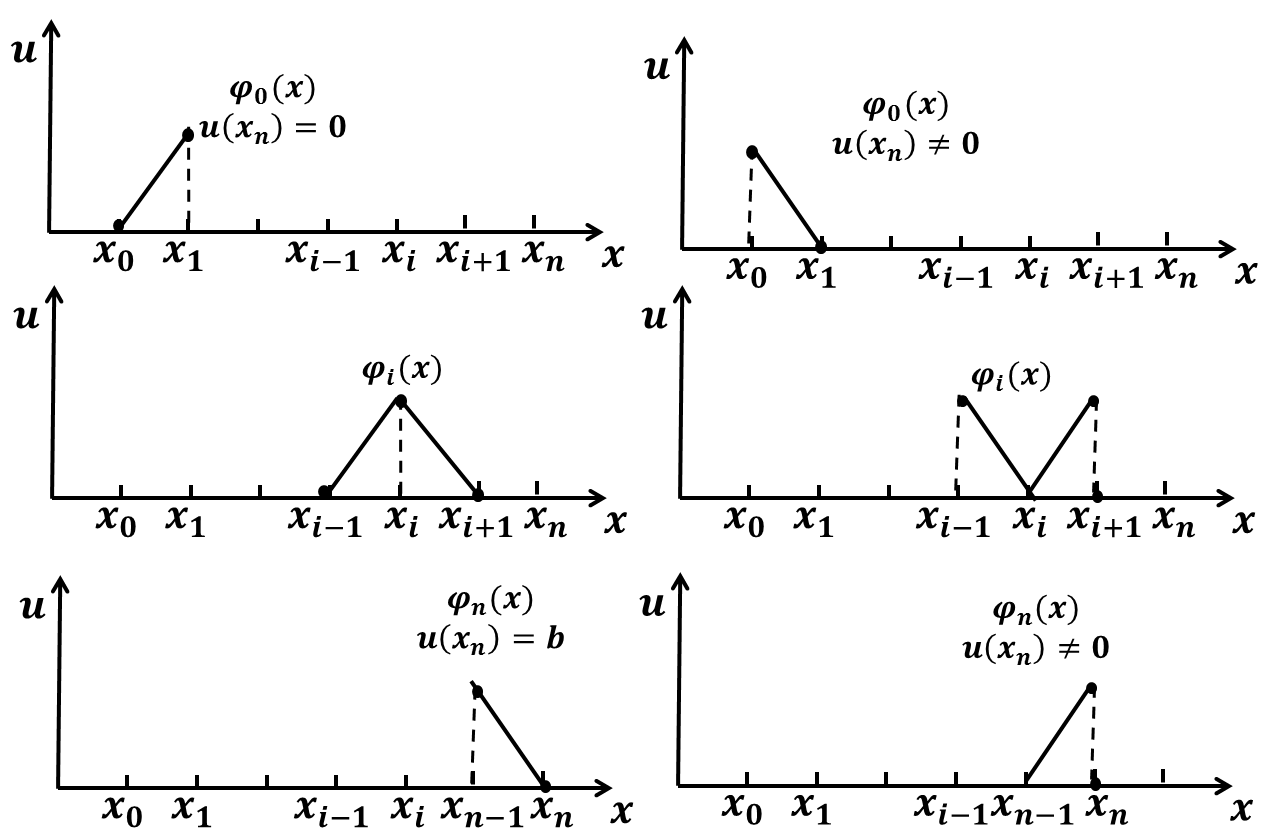
\includegraphics[width=8cm]{images/Piecewise_linear_basis_func.jpg}
        \caption{分段线性的基函数示意图}
        \label{fig:分段线性的基函数示意图}
        \end{figure}
            下面,考虑基的一个具体形式(边值不为0)
            \begin{align*}
                \varphi_0(x) =
                \left \{
                    \begin{aligned}
                        &1 + \frac{x_1 - x}{h_1} , \quad &x_0 \leqslant x \leqslant x_1 \\
                        &0,\quad &\text{其它}
                    \end{aligned}
                 \right.
            \end{align*}
            \begin{align*}
                \varphi_i(x) =
                \left \{
                    \begin{aligned}
                        &1 + \frac{x - x_i}{h_i} , \quad &x_{i-1} \leqslant x \leqslant x_{i } \\
                        &1 + \frac{x - x_i}{h_{i+1}} , \quad &x_{i} \leqslant x \leqslant x_{i + 1} \\
                        &0, \quad &\text{其它}
                    \end{aligned}
                 \right.
            \end{align*}
            \begin{align*}
                \varphi_0(x) =
                \left \{
                    \begin{aligned}
                        &1 + \frac{x - x_n}{h_n} , \quad &x_{n - 1} \leqslant x \leqslant x_n \\
                        &0,  \quad &\text{其它}
                    \end{aligned}
                 \right.
            \end{align*}
            \par
            基于上面这种基$\{\varphi _i\}$,有限维空间$U_n$中的任意一个分段一次多项式$u_h,(u_h \in U_n)$都可以用基函数表示
            \begin{align*}
                u_h(x) = \sum _{i = 1}^n \varphi_i u_i
            \end{align*}
            其中:我们可以看到函数$u_h(x)$在点$x_i$的函数值为$u_i = u_h(x_i)$。
            \par
            至此,我们已经构建了一个有限维空间$U_n$,以及它的基组$\{\varphi _i\}$,我们可以沿用Golerkin方法得到最终的参数值$\{u _i\}$。
            \par
            设$u$是G变分问题的解,$v$为$U$中的任意函数,我们将它们用基函数估计$u,v$,有
            \begin{align*}
                u_h(x) = \sum_{j = 1}^n u_j \varphi_j(x)\\
                v_h(x) = \sum_{j = 1}^n v_i \varphi_i(x)
            \end{align*}
            其中:$u_h,v_h$是$u,v$有限维空间中的估计。将上式带入到G变分问题当中,我们就可以形成如下方程组,解之,即可得到$\{u _i\}$。
            \begin{align*}
                            &\sum_{i = 1}^n a(\varphi_i,\varphi_i)u_i - (f,\varphi_j) = 0 ,\quad j = 1,2,\dots,n\\
                \implies {} &\sum_{i = 1}^n a(\varphi_i,\varphi_j)u_i = \int_a^bf \varphi_j \mathrm{d}x ,\quad j = 1,2,\dots,n
            \end{align*}
            \par
            在实际处理过程中,我们并不把方程中系数矩阵的每个元素$a(\varphi_i, \varphi_j)$按$i$和$j$的顺序依次计算,而是逐元计算其积分值,再累加起来的到系数矩阵。


        \subsubsection{有限元计算步骤}
            \label{subsubsec:有限元计算步骤}
            上面在常微边值问题的基础上介绍了有限元方法,下面用二维泊松方程来介绍有限元的计算步骤,为了便于理解,我们对泊松方程进行简化,并采用三角形元来进行说明。
            \begin{align}
                \label{有限元计算步骤示意的原方程}
                \left\{
                \begin{aligned}
                &Lu: = - \triangle u = f\\
                &u \bigl|_{\partial \Omega} = g
                \end{aligned}
                 \right.
            \end{align}
            为了简单,不妨令$f = x$,$g= 0$,$\Omega$为$(0,-1),(0,1),(1,0)$构成的闭三角区域。
            \paragraph{1.区域$\Omega$离散化}
            我们将$\Omega$离散化为三角形元集合,如图(\ref{fig:三角形元划分示意图}),并设$N_e$为三角形元的个数,$e_k,(k = 1,2,\dots,N_e)$为第$k$个三角形元(单元$k$)。$e_k$有三个端点,分别记为$P_i,P_j,P_k$,$i,j,k$为逆时针方向,则$e_k$可以表示为$e_k(i,j,k)$。我们记$N_p$为端点数。\\
            \begin{figure}[H]
            \centering
            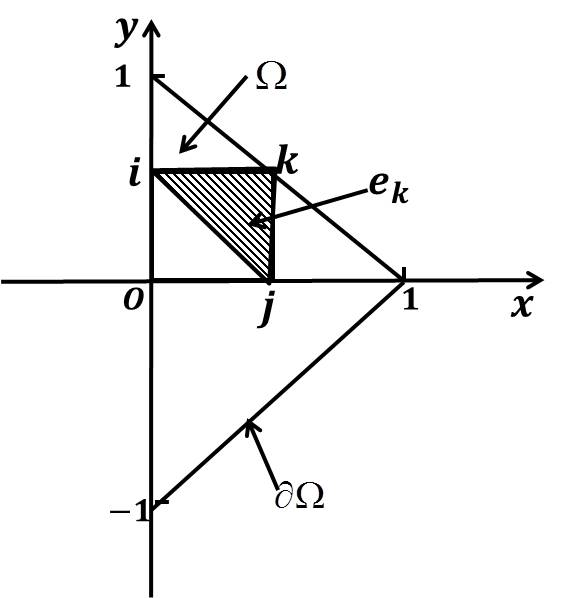
\includegraphics[width=4cm]{images/Triangle_element_division.jpg}
            \caption{三角形元划分示意图}
            \label{fig:三角形元划分示意图}
            \end{figure}
            % \textcolor[rgb]{1 0 0 }{todo:图片:三角形元划分示意图}。\\
            \paragraph{2.选择近似函数}
            在小单元$e_k(i,j,k)$上进行插值,这里,我们选取线性插值,即
            \[
                u_h(x,y) := u_e(x,y) = ax+by+c
            \]
            其中:$a,b,c$为待定系数。
            \paragraph{3.求解单元参数}
            设$u_e(x,y)$在小单元$e_k$在$i,j,k$三点上的函数值为$u_i,u_j,u_k$,则我们可以建立下列方程组
            \begin{align}
                \label{单元方程组}
                \left\{
                    \begin{aligned}
                        &u(x_i,y_i) = ax_i+by_i+c =:u_i\\
                        &u(x_j,y_j) = ax_j+by_j+c =:u_j\\
                        &u(x_k,y_k) = ax_k+by_k+c =:u_k
                    \end{aligned}
                \right.
            \end{align}
            解上述方程组(\ref{单元方程组}),有
            \begin{align}
                \left\{
                    \begin{aligned}
                        &a = \frac{1}{2\Delta e_k} (a_iu_i + a_ju_j+  a_k u_k)\\
                        &b = \frac{1}{2\Delta e_k} (b_iu_i + b_ju_j+  b_k u_k)\\
                        &c = \frac{1}{2\Delta e_k} (c_iu_i + c_ju_j+  c_k u_k)\\
                    \end{aligned}
                \right.
            \end{align}
            其中:$\Delta e_k$为小单元$e_k$的面积
            \begin{align*}
                \Delta e = \frac{1}{2}
                    \begin{vmatrix}
                        x_i &y_i & 1\\
                        x_j &y_j & 1\\
                        x_k &y_k & 1
                    \end{vmatrix}
            \end{align*}

            \begin{align*}
            \left\{
            \begin{aligned}
                &a_i =
                    \begin{vmatrix}
                        y_j & 1\\
                        y_k & 1
                    \end{vmatrix},
                a_j =
                    \begin{vmatrix}
                        y_k & 1\\
                        y_i & 1
                    \end{vmatrix},
                a_k =
                    \begin{vmatrix}
                        y_i & 1\\
                        y_j & 1
                    \end{vmatrix} \\
                &b_i = -
                    \begin{vmatrix}
                        x_j & 1\\
                        x_k & 1
                    \end{vmatrix},
                b_j = -
                    \begin{vmatrix}
                        x_k & 1\\
                        x_i & 1
                    \end{vmatrix},
                b_k = -
                    \begin{vmatrix}
                        x_i & 1\\
                        x_j & 1
                    \end{vmatrix} \\
                &c_i =
                    \begin{vmatrix}
                        x_j & y_j\\
                        x_k & y_k
                    \end{vmatrix},
                c_j =
                    \begin{vmatrix}
                        x_k & y_k\\
                        x_i & y_i
                    \end{vmatrix},
                c_k =
                    \begin{vmatrix}
                        x_i & y_i\\
                        x_j & y_j
                    \end{vmatrix}
            \end{aligned}
            \right.
            \end{align*}
            将$a_1,a_2,a_3$带回$u_e(x,y)$,有
            \[
                u_e(x,y) = N_i(x,y)u_i + N_j(x,y)u_j + N_k(x,y)u_k
            \]
            其中:$N_i(x,y),N_j(x,y),N_k(x,y)$为
            \begin{align}
                \label{向量N的计算}
                \left\{
                \begin{aligned}
                    &N_i(x,y) = \frac{1}{2\Delta e} (a_ix + b_i y+c_i) \\
                    &N_j(x,y) = \frac{1}{2\Delta e} (a_jx + b_j y+c_j) \\
                    &N_k(x,y) = \frac{1}{2\Delta e} (a_kx + b_k y+c_k)
                \end{aligned}
                \right.
            \end{align}
            为了便于书写,我们引入向量
            \begin{align*}
                &\mathbf{N} = [N_i(x,y) + N_j(x,y) + N_k(x,y)] \\
                &\mathbf{u}_e = [u_i,u_j,u_k] ^\mathrm{T}
            \end{align*}
            则$u_e(x,y)$可以写为
            \[
                u_e(x,y) = \mathbf{N}\mathbf{u}_e
            \]
            并且$u_e(x,y)$的梯度可以表示为
            \begin{align*}
                \nabla u_e =
                \left[
                \begin{aligned}
                    \frac{\partial u_e}{\partial x} \\
                    \frac{\partial u_e}{\partial y}
                \end{aligned}
                \right]
                =\mathbf{B} \mathbf{u}_e
            \end{align*}
            其中:
            \begin{align*}
                \mathbf{B}
                &=
                \left[
                \begin{aligned}
                    \frac{\partial N_i}{\partial x} \quad \frac{\partial N_j}{\partial x} \quad \frac{\partial N_k}{\partial x}\\
                    \frac{\partial N_i}{\partial y} \quad\frac{\partial N_j}{\partial y} \quad \frac{\partial N_k}{\partial y}
                \end{aligned}
                \right] \\
                &=
                \frac{1}{2\Delta e_k}
                \left[
                \begin{aligned}
                    a_i \quad a_j \quad a_k\\
                    b_i \quad b_j \quad b_k\\
                \end{aligned}
                \right]
            \end{align*}
            \paragraph{4.构造有限维空间的基函数}
            前面,我们假设函数$u$在单元$e_k$上是线性的,从而构建了函数$u$的有限维空间$U_h$,$U_h$是连续分片线性函数集。$U_h$中的每一个连续分片线性函数都可以由其基组$\{\varphi_i\}$表示。这里,我们考虑高度为1的“角锥函数”为基函数$\varphi_i(i = 1,2,\dots,N_p)$,这样,$U_h$就是一个$N_p$维的有限维空间,其中的函数$u_h(x,y)\in U_h$表示为
            \[
                u_h(x,y) = \sum_{i = 1}^{N_p} u_i\varphi_i(x,y)
            \]
            其中,$u_i$为待求系数。
            \paragraph{5.构建有限元方程}
            原方程(\ref{有限元计算步骤示意的原方程})的G变分问题为:求$u(x,y)$使得
            \begin{align}
                \label{无穷维变分问题}
                a(u,v) = (f,v),\quad \forall v\in U
            \end{align}
            \par
            现在,将函数空间$U$变为有限维空间$U_h$,并且还给出了它的基组,我们用$u_h,v_h$来代替$u,v$
            \begin{align*}
                &u_h(x,y) = \sum_{i = 1}^{N_p} u_i\varphi_i(x,y)\\
                &v_h(x,y) = \sum_{i = 1}^{N_p} v_i\varphi_i(x,y)
            \end{align*}
            则上述无穷维变分问题(\ref{无穷维变分问题})变为有穷维变分问题:求$\{u_i\}$,使得$\forall v_h \in U_h$,有
            \begin{align}
                \label{有限元方程}
                &a(u,v) = (f,v),\quad \forall v\in U\notag\\
                \implies {} &a(u_h,v_h) = (f,v_h),\quad \forall v_h\in U_h \notag\\
                \implies {} &\iint_{\Omega} \nabla u_h \nabla v_h \mathrm{d}x\mathrm{d}y =
                \iint_{\Omega} f v_h \mathrm{d}x\mathrm{d}y ,\quad \forall v_h\in U_h\notag\\
                \implies {} &\sum _{k = 1}^{N_e} \iint\limits_{e_k} \nabla u_h \cdot \nabla v_h \mathrm{d}x\mathrm{d}y =
                \sum _{k = 1}^{N_e} \iint\limits_{e_k} f v_h \mathrm{d}x\mathrm{d}y ,\quad \forall v_h\in U_h
            \end{align}
            上面的计算过程是先逐元计算积分,然后再叠加求和。下面,我们就来计算一下逐元积分,以及它们的和。
            \paragraph{6.单元积分}
            不失为一般性,我们在单元$e_k(i,j,k)$上进行分析。设$u,v$函数在三个定点$P_i,P_j,P_k$上的数值分别为
            \begin{align*}
                \mathbf{u}_e = [u_i,u_j,u_k]^\mathrm{T}\\
                \mathbf{v}_e = [v_i,v_j,v_k]^\mathrm{T}
            \end{align*}
            则在$e_k$上,有
            \begin{align*}
                \left\{
                \begin{aligned}
                    &u_e(x,y) = \mathbf{N} \mathbf{u}_e\\
                    &v_e(x,y) = \mathbf{N} \mathbf{v}_e\\
                    &\nabla u_e = \mathbf{B} \mathbf{u}_e\\
                    &\nabla v_e = \mathbf{B} \mathbf{v}_e
                \end{aligned}
                \right.
            \end{align*}
            于是单元$e_k$上的积分$\iint_{e_k} \nabla u_h \nabla v_h \mathrm{d}x\mathrm{d}y$和$\iint_{e_k} f v_h \mathrm{d}x\mathrm{d}y$是可以计算的
            \begin{align*}
                \iint\limits_{e_k} \nabla u_h \cdot \nabla v_h \mathrm{d}x\mathrm{d}y
                &=\iint\limits_{e_k} (\nabla v_h)^\mathrm{T} (\nabla u_h ) \mathrm{d}x\mathrm{d}y\\
                &=\iint\limits_{e_k} (\mathbf{B} \mathbf{v}_e)^\mathrm{T} (\mathbf{B} \mathbf{u}_e) \mathrm{d}x\mathrm{d}y\\
                & = \mathbf{v}_e^\mathrm{T} \overline{\mathbf{K}}_e \mathbf{u}_e
            \end{align*}
            其中:
            \begin{align*}
                \overline{\mathbf{K}}_e &= \iint\limits_{e_k} \mathbf{B}^\mathrm{T} \mathbf{B} \mathrm{d}x\mathrm{d}y \\
                &=\mathbf{B}^\mathrm{T} \mathbf{B} \iint\limits_{e_k} \mathrm{d}x\mathrm{d}y \\
                &=\Delta e_k\mathbf{B}^\mathrm{T} \mathbf{B}\\
                &=\frac{1}{4 \Delta e_k}
                    \begin{bmatrix}
                        a_i & b_i\\
                        a_j & b_j\\
                        a_k & b_k\\
                    \end{bmatrix}
                    \begin{bmatrix}
                        a_i & a_j & a_k\\
                        b_i & b_j & b_k\\
                    \end{bmatrix}
            \end{align*}
            $\Delta e_k$为小单元$e_k$的面积。
            \par
            我们将$\overline{\mathbf{K}}_e$记为
            \begin{align*}
                \overline{\mathbf{K}}_e =
                \begin{bmatrix}
                    \bar{k}_{ii} & \bar{k}_{ij} & \bar{k}_{ik} \\
                    \bar{k}_{ji} & \bar{k}_{jj} & \bar{k}_{jk} \\
                    \bar{k}_{ki} & \bar{k}_{kj} & \bar{k}_{kk} \\
                \end{bmatrix}
            \end{align*}
            其中:
            \[
            \bar{k}_{st} = \frac{1}{4\Delta e_k}(a_sa_t + b_sb_t) \quad s,t = i,j,k
            \]
            称$\overline{\mathbf{K}}_e$为单元刚度矩阵。
            \par
            同理,我们来处理另一个单元积分
            \begin{align*}
                \iint\limits_{e_k} f v_h \mathrm{d}x\mathrm{d}y
                &=\iint\limits_{e_k} (\mathbf{N}\mathbf{v}_e)^\mathrm{T} f\mathrm{d}x\mathrm{d}y\\
                &=\iint\limits_{e_k} \mathbf{v}_e^\mathrm{T}\mathbf{N}^\mathrm{T} f\mathrm{d}x\mathrm{d}y\\
                & = \mathbf{v}_e^\mathrm{T}\overline{\mathbf{F}}_e
            \end{align*}
            其中:向量$\mathbf{N}$的计算如公式(\ref{向量N的计算}),
            \begin{align*}
                \overline{\mathbf{F}}_e = \iint\limits_{e_k} \mathbf{N}^\mathrm{T} f\mathrm{d}x\mathrm{d}y =
                \begin{bmatrix}
                    \bar{F}_i\\\bar{F}_j\\\bar{F}_k
                \end{bmatrix}
            \end{align*}
            \begin{align*}
                \bar{F}_j = \iint\limits_{e_k} \mathbf{N}_s f\mathrm{d}x\mathrm{d}y \quad s = i,j,k
            \end{align*}
            \[
                N_i(x,y) = \frac{1}{2\Delta e} (a_ix + b_i y+c_i)
            \]
            我们称$\overline{\mathbf{F}}_e$为单元载荷向量。
            \paragraph{7.单元积分求和}
            在计算完单元$e_k$上的积分$\iint_{e_k} \nabla u_h \nabla v_h \mathrm{d}x\mathrm{d}y$和$\iint_{e_k} f v_h \mathrm{d}x\mathrm{d}y$之后,我们要将所有单元的积分相加,即计算$\sum\limits_{k= 1}^{N_e }\iint\limits_{e_k}(\cdot)$。
            \par
            对某个小单元$e_k$来说,端点$i,j,k$是逆时针排列的,但是,这只是在一个小单元里的标记,每个节点在的$N_p$个节点中有着$1 - N_p$的编号。令
            \begin{align*}
                &\mathbf{v}_e = [v_i,v_j,v_k]^\mathrm{T} = \mathbf{C}_e\mathbf{v}\\
                &\mathbf{u}_e = [u_i,u_j,u_k]^\mathrm{T} = \mathbf{C}_e\mathbf{u}
            \end{align*}
            其中:$\mathbf{C}_e$是一个$3\times N_p$的$0,1$指示矩阵。$\mathbf{C}_e$在第一行对应$i$的列、第二行对应$j$的列、第三行对应$k$的列上的矩阵元素为$1$,其余矩阵元素为$0$,$\mathbf{v} = [v_i,v_j,v_k]$。
            \par
            这样,我们有
            \begin{align}
                \label{单元积分求和1}
                   &\sum\limits_{k= 1}^{N_e }\iint\limits_{e_k}\nabla u_h \nabla v_h \mathrm{d}x\mathrm{d}y \notag \\
                ={}&\sum\limits_{k= 1}^{N_e }\mathbf{v}_e^\mathrm{T} \overline{\mathbf{K}}_e\mathbf{u}_e\notag \\
                ={}&\sum\limits_{k= 1}^{N_e }\mathbf{v}^\mathrm{T} \mathbf{C}_e^\mathrm{T}\overline{\mathbf{K}}_e \mathbf{C}_e \mathbf{u}\notag \\
                ={}&\mathbf{v}^\mathrm{T} \mathbf{K}\mathbf{u}
            \end{align}
            其中:$\mathbf{K} = \sum\limits_{k= 1}^{N_e }\mathbf{C}_e^\mathrm{T}\overline{\mathbf{K}}_e \mathbf{C}_e$。
            \par
            我们称$\mathbf{K}$为总刚度矩阵。同理,可以处理下一个单元累加
            \begin{align}
                \label{单元积分求和2}
                   &\sum\limits_{k= 1}^{N_e }\iint\limits_{e_k}f \nabla v_h \mathrm{d}x\mathrm{d}y \notag \\
                ={}&\sum\limits_{k= 1}^{N_e }\mathbf{v}_e^\mathrm{T} \overline{\mathbf{F}}_e \notag \\
                ={}&\sum\limits_{k= 1}^{N_e }\mathbf{v}^\mathrm{T} \mathbf{C}_e^\mathrm{T}\overline{\mathbf{F}}_e \notag \\
                ={}&\mathbf{v}^\mathrm{T} \mathbf{F}
            \end{align}
            其中:$\mathbf{F} = \sum\limits_{k= 1}^{N_e }\mathbf{C}_e^\mathrm{T}\overline{\mathbf{F}}_e $。
            我们称$\mathbf{F}$为总载荷矩阵。
            \paragraph{8.求解有限元方程组}
            我们将(\ref{单元积分求和1})和(\ref{单元积分求和2})带入到有限元方程(\ref{有限元方程}),有
            \begin{align*}
                &\sum _{k = 1}^{N_e} \iint\limits_{e_k} \nabla u_h \cdot \nabla v_h \mathrm{d}x\mathrm{d}y =
                    \sum _{k = 1}^{N_e} \iint\limits_{e_k} f v_h \mathrm{d}x\mathrm{d}y ,\quad \forall v_h\in U_h \\
                \implies {} &\mathbf{v}^\mathrm{T} \mathbf{K}\mathbf{u} = \mathbf{v}^\mathrm{T} \mathbf{F} ,\quad \forall \mathbf{v}\in R^{N_p}  \\
                \implies {} &\mathbf{v}^\mathrm{T}(\mathbf{K}\mathbf{u} -  \mathbf{F}) = 0,\quad \forall \mathbf{v}\in R^{N_p}
            \end{align*}
            由此,我们得到$\mathbf{u}$ 的方程组
            \begin{align*}
                \mathbf{K}\mathbf{u} -  \mathbf{F} = 0
            \end{align*}
            解上述方程组后即可得到$\mathbf{u}$,$\mathbf{u}$的分量$u_1,u_2,\dots,u_{N_p}$即为函数$u_h(x,y)$在网格点$1$到$N_p$各点的函数值,即$u(x,y)$的数值估计。之后,我们有函数$u_h(x,y) = \sum_{i  =1}^{N_p} u_i \varphi_i(x,y)$,$i = 1,2,\dots,N_p$为定点。\\
           注:在上述求解过程中,我们考虑的是二维泊松方程的第一边值条件,并且假设边值条件为$0$,即$g = 0$。关于更一般的边值条件可参考其它书籍,如《偏微分方程数值解法(第二版)》陆金甫P228。
           \par
           考虑:1、上面的讨论是用三角形元对区域$\Omega$进行划分的,是否可以考虑其它元,比如:长方形元。2、上面假设$u(x,y)$在小单元$e_k$上是一次函数,能否考虑高次函数,比如:二次函数。

    \subsection{谱分析方法}
        \subsubsection{有限元法和谱方法的讨论}
            \label{subsubsec:有限元法和谱方法的讨论}
            \par
            下面,我们在一维情况下讨论有限元方法和谱方法。考虑如下两个问题\\
            问题1:回归(拟合问题)。根据测量数据$\{x_i\,y_i\}_{i = 1}^m$,求回归函数$y = f(x),a<x<b$。\\
            问题2:常微分方程问题。求函数$y = f(x)$,满足如下常微分方程
            \begin{align*}
            \left\{
                \begin{aligned}
                    &y' = g(y,x)\\
                    &y(a) = \alpha\\
                    &y(b) = \beta
                \end{aligned}
            \right.
            \end{align*}
            \par
            上述两个问题都是在二维平面域$xOy$上求函数$y = f(x)$,问题1要求$y(x)$距离真实数据点$\{x_i\,y_i\}_{i = 1}^m$合理,问题2要求$y(x)$满足方程。下面,不要考虑回归,也不要考虑ODE,我们来自己找一个函数$y(x)$,到平面域上去找,可以有无数种可选择的函数$f_1,f_2,\dots,f_n,\dots$。定义在区间域$I= [a,b]$内所有函数的集合为$\varPhi_f$,$\varPhi_f$中包含了各种各样的函数:处处可微的、光滑的、分段的、处处不可导的、无穷大的。显然,我们不能在无穷维函数空间$\varPhi_f$中一个一个函数的找,那太恐怖了,也是不现实的。我们要在$\varPhi_f$的子空间(子集or子域)中寻找$f$。显然,应该把那些值无穷的函数类去掉,但仅仅如此还是不够的,我们不妨要求$f$具有特征:光滑或者可积或者平方可积或者分段或者其它,记这样的特征函数集合为$H = \{f|\text{特征}\}$。先不讨论$H$,我们继续看,如果$f$是解,那么我们可以称$H$为特征可行域,但在$H$中找$f$仍然不太现实,例如在$I$上的平方可积的函数有无穷多个,$H$仍然是一个无穷维空间,$(f_1,f_2,\dots,f_n,\dots) = \{f\}^\infty$,既然如此,我们不妨将空间$H$进一步缩小,比如我们考虑如下的$n$次多项式函数空间$H_n$
            \begin{align}
                \label{n次多项式函数集}
                H_n = \left\{
                    \begin{aligned}
                        &f_1(x) = ax+b\\
                        &f_2(x) = ax^2+bx+c\\
                        &\qquad \quad \vdots \\
                        &f_n(x) = a x_n+bx_{n-1}+\dots
                    \end{aligned}
                \right.
            \end{align}
            我们就在$H_n$中找$f$,看哪一个$f$相对而言最好(满足一定的指标)。现在好了,$H_n$是空间$H$的一个有限维子空间,是可以搜索的,我们称$H_n$为函数$f$的探索空间(前面记为$U_n$)。对一个小的$H_n$而言,我们可以将其中的元素$f$列举出来,但对于一个大空间,就无能为力了。考虑到三维空间中的任一向量可以由基向量表示,那么,我们能不能找到$H_n$中的基函数$\{\varphi_i\}$,使$H_n$中的所有函数$f_i\in H_n$都可以用基函数表示?可以的,比如上面的$n$次多项式函数集(\ref{n次多项式函数集})$H_n$中的任意一个函数$f_i$都可以用$\{x^0,x^1,x^2,\dots,x^n\}$表示
            \begin{align*}
                f = \sum_{i = 0}^n c_ix^i
            \end{align*}
            其中:$c_i$为待求系数。
            \par
            我们将$\{x^0,x^1,x^2,\dots,x^n\}$作为基组,$\{\varphi_i\}_{i = 1}^n = \{x^0,x^1,x^2,\dots,x^n\}$,并称$H_n$是基组$\{\varphi_i\}_{i = 1}^n$张成的探索空间,记为
            \begin{align*}
                H_n = \mathbf{span} \{\varphi_1,\varphi_2,\dots,\varphi_n\}
            \end{align*}
            其中:$n$为基组中基函数的个数。
            \par
            同一空间中的基组有不同的形式(即基组不唯一),并且,观察到三维空间$Oxyz$的基向量$\vec{e}_1,\vec{e}_2,\vec{e}_3$两两之间相互垂直,为正交基向量(正交基底),我们也可以在$H_n$中选择正交基组$\{\varphi_i\}_{i = 1}^n$:$\forall i,j \in n$,$i\neq j$,$\varphi_i,\varphi_j\in \{\varphi_i\}_{i = 1}^n$,有
            \[
                \int_a^b \varphi_i\varphi_j \mathrm{d}x = 0
            \]
            由此,我们有$H_n$在$I = [a,b]$上的正交基组。
            \par
            仔细看$f = \sum_{i = 0}^n c_ix^i$,这很像傅里叶级数,我们来回顾一下傅里叶级数:将$f(x)$在区间$[-\pi,\pi]$上展开,有
            \begin{align*}
                \hat{f}(x) = \frac{a_0}{2} + \sum _{k = 1} ^\infty (a_k\cos kx + b_k\sin kx)
            \end{align*}
            其中:
            \begin{align*}
            \left\{
                \begin{aligned}
                    &a_0 = \frac{1}{\pi} \int_{-\pi }^\pi f(x) \mathrm{d}x\\
                    &a_n = \frac{1}{\pi} \int_{-\pi }^\pi f(x) \cos nx \mathrm{d}x\\
                    &b_n = \frac{1}{\pi} \int_{-\pi }^\pi f(x) \sin nx\mathrm{d}x\\
                \end{aligned}
            \right.
            \end{align*}
            \par
            $\hat{f}(x)$为函数$f(x)$的逼近(估计),$f(x) \sim \hat{f}(x)$,当然我们要判断$\hat{f}(x)$的收敛性,这里我们不做讨论。可以看到$f(x)$在$[-\pi ,\pi]$上被展成了$\{1,\cos x,\sin x,\cos 2x,\sin 2x,\dots,\cos nx,\sin nx\}$的线性组合的形式,所以$\{1,\cos x,\sin x,\cos 2x,\sin 2x,\dots,\cos nx,\sin nx\}$是$H_n$的一个基组,并且该基组是正交基组,因为$\forall i,j \in n$,$i\neq j$,有
            \begin{align*}
                \left\{
                    \begin{aligned}
                        &\int_{-\pi }^\pi \cos (ix)\sin(jx) \mathrm{d}x = 0\\
                        &\int_{-\pi }^\pi \cos (ix)\cos(jx) \mathrm{d}x = 0\\
                        &\int_{-\pi }^\pi \sin (ix)\sin(jx) \mathrm{d}x = 0\\
                        &\int_{-\pi }^\pi \cos(ix) \mathrm{d}x = 0\\
                        &\int_{-\pi }^\pi \sin(ix) \mathrm{d}x = 0\\
                    \end{aligned}
                \right.
            \end{align*}
            即基组中的任意两个不同的基函数的区间卷积为$0$。
            \par
            在这一章后面,我们会讨论一些其它形式的正交基,如:Legendre多项式、Chebushev多项式、Hermite多项式、Jacobi多项式、Laguerre多项式等。
            \par
            在选取基组$\{\varphi_i\}$时,我们自然希望由$\{\varphi_i\}$张成的空间$H_n$尽可能大。现在,回到我们的问题当中,设要求解的函数为$u$(一维空间为$u(x)$,二维空间为$u(x,y)$),设其自变量区域为$\Omega$,区域边界$\partial \Omega$,探索空间为$U_n$(前面写为$H_n$),$U_n$的基组为$\{\varphi_i\}_{i = 1}^n$,我们的目标是在$U_n$中寻找$u(x)$的替代(估计)$u_n(x)$。由于$u_n(x)$可以由基组表示
            \[
                u_n(x) = \sum_{i = 1}^n c_i \varphi_i(x)
            \]
            那么,寻找$u_n(x)$的过程就变为寻找系数$c_i$的过程,这样,我们就把泛函极值问题变为了参数极值问题。
            \par
            如果对$u(x)$的要求不同(如$u(x)$不必处处可微),那么探索空间$U_n$就会不同,从而基组$\{\varphi_i\}$就不同,前面说到,我们希望$U_n$尽可能大。\ding{172}一种想法是假设$U_n(x)$为分段多项式形式,$u_n(x)\in U_n$在$I=[a,b]$上可以是分段一次多项式,也可以是二次和更多次的,分段多项式次数不同,基组也就不同。不妨设$u_n(x)$在$I$上为分段一次多项式,将$I$离散化为$n$段,并且有$n$个基函数$\varphi_i(x)$。如果基函数$\varphi_x(x)$在$x_i$处的函数值为$1$,其它基函数在$x_i$处的函数值为$0$。那么,基函数的系数$c_i$就可以写为函数值$u_i$,这样,最终求得的$\{u_i\}$即为$u(x)$的数值解,这正是有限元的思想。\ding{173}另一种想法是假设$U_n(x)$在$\Omega$内光滑或者无穷次可微,设探索空间为$U_n = \{u_n(x)|\text{特征}\}$,基组为$\{\varphi_i\}$,则函数$u_n(x)$可以表示为
            \[
                u_n(x) = \sum_{i = 1}^n c_i \varphi_i(x)
            \]
            于是求$u_n(x)$就变为求$c_i$,取不同基组$\{\varphi_i\}$,可以得到不同结果,这是谱分析的思想。比较有限元方法和谱方法,有限元方法以分段函数(集)作为探索空间,以分段函数作为基组;谱方法以整体无限光滑的函数集作为探索空间,以无限光滑函数作为基组(如Legendre多项式、Chebushev多项式、Hermite多项式、Jacobi多项式、Laguerre多项式等)。
            \subsubsection{周期边值问题的谱方法}
                \label{subsubsec:周期边值问题的谱方法}
                \par
                上面介绍了有限元方法和谱方法的思想,下面,我们来具体介绍谱方法。谱方法和有限元方法都是基于R-G方法的,谱方法有Galerkin谱方法、Tau方法和配点法(拟谱方法)之分,在后面的嫦娥3号登月的建模中,我们介绍了配点法,这里就不再重述了。其实,谱方法的思想来源已久,早在1820年,Navier就用谱方法的思想求解了弹性薄板问题,但是很长一段时间内,谱方法由于计算量大,在边界处要满足条件等劣势而没有被广泛应用。1965年,快速傅里叶变换FFT的出现使谱方法得以重获新生。近30年来,谱方法更是快速发展起来,值得注意的是,谱方法的基函数是一个定义在$n$维长方体上的正交多项式,因此,谱方法要求求解的区域$\Omega$满足一定的条件。将谱方法用于更广泛的区域$\Omega$形式是一项值得研究的工作,
                \par
                前面,我们提到过,谱方法的探索函数$u_n(x)$被取为无穷可微函数,Galerkin谱方法的检验函数$v_n(x)$与试探函数$u_n(x)$属于同一空间$U_n$,并在边界处满足条件,Tau方法则不要求$v_n(x)$满足边界条件。用Galerkin谱方法求解如下周期边值问题
                \begin{align}
                    \label{周期边值问题}
                    \left\{
                        \begin{aligned}
                            &Lu:= - u'' = f(x)\\
                            &u(0) = u(2\pi) = 0\\
                            &x\in [0,2\pi]
                        \end{aligned}
                    \right.
                \end{align}
                用$v$乘上式(\ref{周期边值问题})两边,并在区间$[0,2\pi]$上积分,有
                \begin{align*}
                    \int_0^{2\pi} Lu\ v \mathrm{d}x = \int _0^{2\pi}  f x\mathrm{d}x
                \end{align*}
                然后,对上式左边的积分用分部积分法并结合边值条件,有
                \begin{align*}
                    \int_0^{2\pi} Lu\ v \mathrm{d}x &= \int_0^{2\pi} u' v '\mathrm{d}x - u'v\Bigl|_0^{2\pi} + \int_0^{2\pi} u v \mathrm{d}x\\
                    &=\int_0^{2\pi} u' v '\mathrm{d}x
                \end{align*}
                令
                \begin{align*}
                    &a(u,v) = \int_0^{2\pi} u'v'\mathrm{d}x\\
                    &(f,v) = \int_0^{2\pi} fv\mathrm{d}x
                \end{align*}
                于是原问题(\ref{周期边值问题})的G变分问题为:求$u(x) \in U$,使得对$\forall v \in U, v(0) = v(2\pi) = 0$,有
                \begin{align}
                    \label{G变分问题}
                    a(u,v) = (f,v)
                \end{align}
                \par
                取无穷维空间$U$的有限维探索空间$U_n=\{u_n(x) |\text {特征}\}$,探索空间的基组为$\{\varphi_k\}_{k = -N}^{N}$,基函数的具体形式为
                \[
                    \varphi_k(x) = e^{-ikx} -1 \quad k = \pm 1, \pm 2,\dots,\pm N
                \]
                $U_n$由基组张成,$U_n = \mathbf{span} \{\varphi_k\}_{k = -N}^{N}$。于是,$u_n(x) \in U_n$可以表示成如下的形式
                \begin{align*}
                    u_n(x) = \sum_{k = -N}^{N} c_k \varphi_k = \sum_{k = -N}^{N} c_k (e^{-ikx} -1 )
                \end{align*}
                于是,原变分问题变为求参数$\{c_k\}_{k = -N}^{N}$。我们将$u,v$的估计$u_n(x),v_n(x)$
                \begin{align*}
                    u_n(x) = \sum_{k = -N}^{N} c_k \varphi_k = \sum_{k = -N}^{N} c_k (e^{-ikx} -1 )\\
                    v_n(x) = \sum_{k = -N}^{N} c_j \varphi_j = \sum_{j = -N}^{N} c_k (e^{-ijx} -1 )
                \end{align*}
                带入G变分问题(\ref{G变分问题})中来进行整理,有
                \begin{align}
                    %\label{G变分问题}
                               &a(u,v) = (f,v) \quad \forall v(x)\in  U \notag\\
                    \implies {}&a(u_n,v_n) = (f,v_n)\quad \forall v_n(x) \in U_n
                \end{align}
                由于$v_n(x)$的任意性($\forall v_n(x) \in U_n$),不妨令$v_n(x)$就为空间$U_n$的基函数$\varphi_j(x)$,于是有下面的参数方程
                \begin{align}
                    \label{参数方程}
                               &a(u,v) = (f,v) \quad \forall v(x)\in  U \notag\\
                    \implies {}&a(u_n,\varphi_j) = (f,\varphi_j)
                    \quad \forall \varphi_j(x) \in U_n ,j = \pm 1, \pm 2,\dots,\pm N \notag\\
                    \implies {}&a\left(\sum_{k = -N}^{N} c_k (e^{-ikx} -1 ),\varphi_j\right) = (f,\varphi_j)
                    \quad \forall j = \pm 1, \pm 2,\dots,\pm N \notag\\
                    \implies {}&\sum_{k = -N}^N c_k a\left( e^{-ikx} -1,\varphi_j \right)= (f,\varphi_j)
                    %\quad \forall j = \pm 1, \pm 2,\dots,\pm N
                    \notag\\
                    \implies {}&\sum_{k = -N}^N c_k a\left( e^{-ikx},\varphi_j \right)= (f,\varphi_j)
                    %\quad \forall j = \pm 1, \pm 2,\dots,\pm N
                    \notag\\
                    \implies {}&\sum_{k = -N}^N c_k a\left( e^{-ikx},e^{-ijx} -1 \right)= (f,\varphi_j)
                    %\quad \forall j = \pm 1, \pm 2,\dots,\pm N
                    \notag\\
                    \implies {}&\sum_{k = -N}^N c_k a\left( e^{ikx},e^{ijx} \right) - \sum_{k = -N}^N c_k a\left( e^{-ikx},1 \right)= (f,\varphi_j) \notag \\
                    \implies {}&\sum_{k = -N}^N c_k a\left( e^{ikx},e^{ijx} \right) = (f,\varphi_j)
                    \quad \forall j = \pm 1, \pm 2,\dots,\pm N
                \end{align}
                注意,还有
                \begin{align*}
                    \sum_{k = -N}^N c_k = 0
                \end{align*}
                我们下面的工作就是求$ a\left( e^{ikx},e^{ijx} \right)$和$(f,\varphi_j) $。
                \begin{align}
                    \label{参数方程子式}
                    a\left( e^{ikx},e^{ijx} \right) &= \int_0^{2\pi} e^{ikx} e^{ijx}\mathrm{d}x \notag \\
                    & = \int_0^{2\pi} -(ik)(ij) e^{ikx} e^{-ijx}\mathrm{d}x \notag \\
                    & =
                    \left\{
                    \begin{aligned}
                        2\pi j^2,\quad k = j \\
                        0,\quad k \neq j \\
                    \end{aligned}
                    \right.
                \end{align}
                特别地,当$k = j = 0$时,有$a(1,1) = 0$。将上式(\ref{参数方程子式})带入到参数方程(\ref{参数方程}),对$\forall j = \pm 1, \pm 2,\dots,\pm N$,有
                \begin{align*}
                    a(u_n,\varphi_j)& = \sum_{k = -N}^N c_k a\left( e^{ikx},e^{ijx} \right)=: (f,\varphi_j) \\
                    &=
                    \left\{
                    \begin{aligned}
                        &\sum_{k = -N}^N c_k 2\pi j^2,&\quad k = j \\
                        &\sum_{k = -N}^N c_k 0,&\quad k \neq j \\
                    \end{aligned}
                    \right\}
                     =: (f,\varphi_j) \\
                     & = c_j2\pi(j^2) =: (f,\varphi_j)
                \end{align*}
                \par
                由于$v_n$的任意性($\forall j = \pm 1, \pm 2,\dots,\pm N$),方程中共$2N+1$个参数$\{c_i\}$,所以我们要将$2N$个基函数$\varphi_j$都带入方程,以形成如下$2N+1$个方程组
                \begin{align*}
                    \left\{
                        \begin{aligned}
                            &c_j 2\pi(j^2) = (f,\varphi_j) \quad j = \pm 1, \pm 2,\dots,\pm N\\
                            &\sum_{k = -N}^N c_k = 0
                        \end{aligned}
                    \right.
                \end{align*}
                共有$2N+1$个待求参数$\{c_k\}_{k = -N}^N$,有$2N+1$个方程,解之,可得$\{c_k\}_{k = -N}^N$。
            \subsubsection{正交多项式}
                \label{subsubsec:正交多项式}
                \par
                上面的谱方法是基于常微周期边界的,对于非周期边界,我们用Legendre多项式、Chebyshev多项式等作为基组来进行求解,为此,我们给出Legendre、Chebyshev、Hermite、Jacobi和Laguerre等多项式的定义以及部分性质。在介绍多项式之前,先来定义一下基组中基函数的正交性。
                \paragraph{正交性}设$f,g \in C(I)$,$\rho$是$I= [a,b]$上的权函数,若
                \[
                    (f,g)_\rho = \int_a^b \rho(x)fg\mathrm{d}x = 0
                \]
                则称$f,g$在$I$上带权$\rho$正交。
                \paragraph{Legendre多项式}Legendre多项式是由下列Legendre方程导出的
                \begin{align*}
                    (1 - x^2) y'' -2xy' +n(n+1)y = 0
                \end{align*}
                上述方程的通解为
                \[
                    y(x) = AP_n(x) +BQ_n(x)
                \]
                其中:$A,B$为常数,$P_n,Q_n$分别为第一、第二类Legendre函数。
                \par
                Legendre函数的一般形式为
                \begin{align}
                    \label{eq:Legendre函数的一般形式}
                    &P_n(x) = \sum_{m=0}^{[n/2]} \frac{(-1)^m (2n-2m)!}
                    {2^n m! (n-m)!(n-2m)!} x^{n-2m}
                    \\
                    &Q_n(x) = P_n(x)\int\frac{1}{(1-x^2)P_n^2}\mathrm{d}x \notag
                \end{align}
                其中:$[\cdot]$表示取整。
                \par
                Legendre函数的递推公式为
                \begin{align*}
                &P_0(x) = 1 \\
                &P_1(x) = x \\
                &P_2(x) = \frac{1}{2}(-1+3x^2) \\
                &P_3(x) = \frac{1}{2}(-3x+5x^2) \\
                &P_4(x) = \frac{1}{8}(3-30x^2+34x^4) \\
                &P_5(x) = \frac{1}{8}(15x-70x^3+63x^5) \\
                &\dots \\
                &(n+1)P_{n+1}(x) - (2n+1)xP_n(x)+nP_{n-1}(x)= 0
                \end{align*}
                $n$从$0$到$5$的函数图像如图(\ref{fig:Legendre多项式MATLAB图像})\footnote{https://en.wikipedia.org/wiki/Legendre\_polynomials}所示
                \begin{figure}[H]
                \centering
                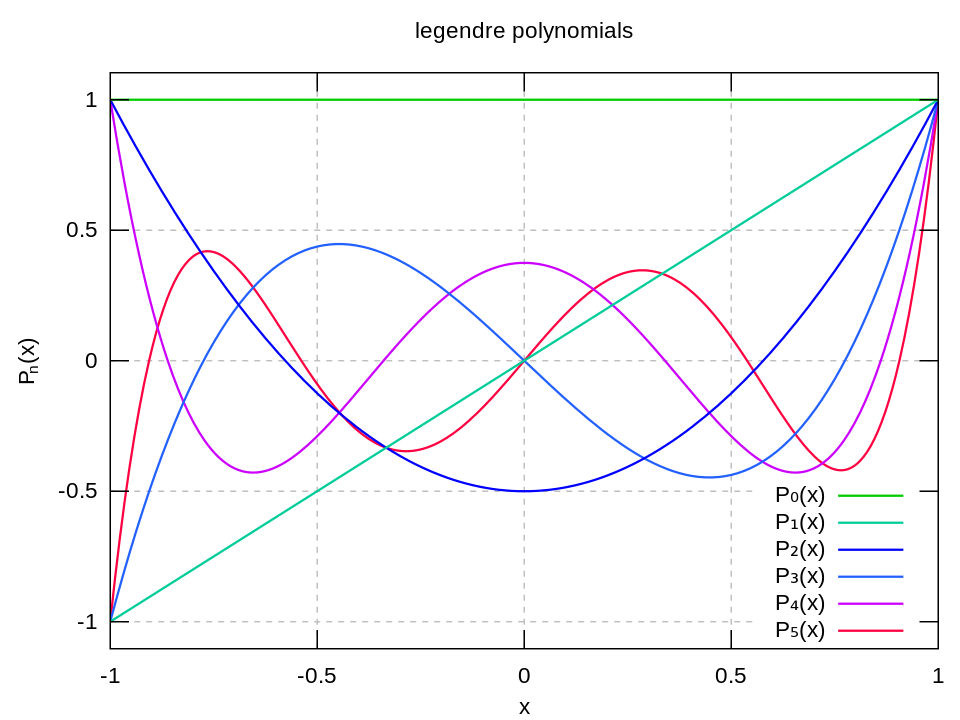
\includegraphics[width=8cm]{images/Legendre_polynomial_matlab_pic.png}
                \caption{Legendre多项式MATLAB图像}
                \label{fig:Legendre多项式MATLAB图像}
                \end{figure}
                % \textcolor[rgb]{1 0 0}{todo:matlab图片:Legendre多项式MATLAB图像}
                \par
                Legendre函数的正交性
                \begin{align*}
                    \int_{-1}^1 P_n(x) P_m(x) \mathrm{d}x =
                    \left\{
                        \begin{aligned}
                            &\frac{2}{2n+1}, & n = m\\
                            &0, & n \neq m\\
                        \end{aligned}
                    \right.
                    = \frac{2}{2n+1} \delta_{mn}
                \end{align*}
                其中:$\delta_{mn}$为示性函数,当$m = n$时才起作用。
                \paragraph{Chebyshev多项式} Chebyshev是下列方程的解
                \begin{align*}
                (1-x^2)y'' - xy' +n^2y = 0
                \end{align*}
                \par
                Chebyshev函数的递推公式为
                \begin{align}
                    \label{Cheby的递推公式}
                    &T_0(x) = 1 \notag \\
                    &T_1(x) = x \notag \\
                    &T_2(x) = 2x^2 - 1 \notag \\
                    &T_3(x) = 4x^3 - 3x \notag \\
                    &T_4(x) = 8x^4 - 8x^2 +1 \notag \\
                    &\dots \notag \\
                    &T_{n+1}(x) = 2xT_n(x) - T_{n-1}(x)
                \end{align}
                $n$取值$0$到$4$时的函数图像如图(\ref{fig:Chebyshev多项式MATLAB图像})\footnote{https://en.wikipedia.org/wiki/Chebyshev\_polynomials}所示
                \begin{figure}[H]
                \centering
                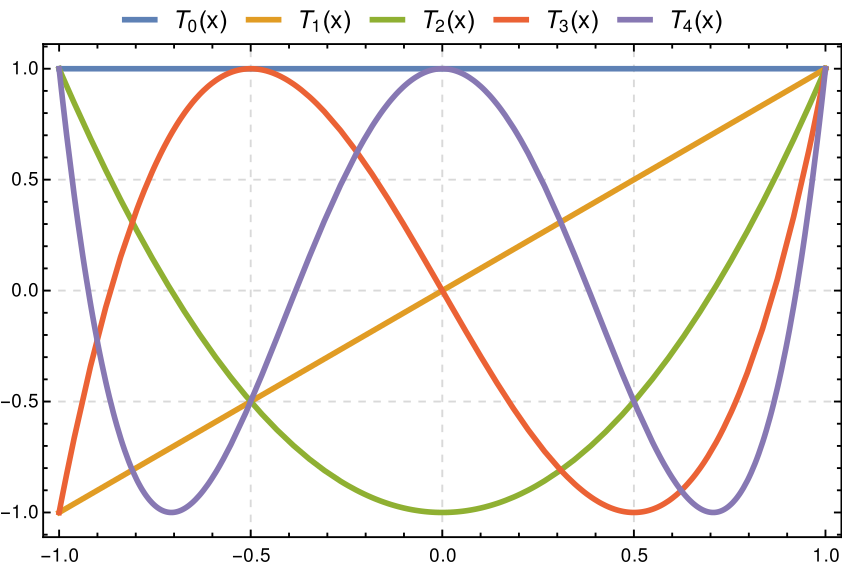
\includegraphics[width=8cm]{images/Chebyshev_polynomial_matlab_pic.png}
                \caption{Chebyshev多项式MATLAB图像}
                \label{fig:Chebyshev多项式MATLAB图像}
                \end{figure}
                % \textcolor[rgb]{1 0 0}{todo:matlab图片:Chebyshev多项式MATLAB图像}
                \par
                注意到三角关系式
                \[
                    \cos((n+1)\theta) + \cos((n-1)\theta) = 2\cos\theta \cos(n\theta)
                \]
                将上式与递推公式(\ref{Cheby的递推公式})比较,当$\theta = \arccos x$时,发现$\cos (x \arccos x)$满足递推关系式,所以有
                \begin{align*}
                    \left\{
                        \begin{aligned}
                            &T_n(x) = \cos n\theta\\
                            &\theta = \arccos x\\
                            &n \geqslant 0\\
                            &x \in I
                        \end{aligned}
                    \right.
                \end{align*}
                \par
                Chebyshev的正交性
                \begin{align*}
                \int _0^{\pi} \cos(m\theta) \cos(n\theta) \mathrm{d}x = 0 \quad m\neq n
                \end{align*}
                或者
                \begin{align*}
                    (T_m,T_n) = \int_{-1}^1 \frac{1}{\sqrt{1-x^2}} T_m(x) T_n(x) \mathrm{d}x = 0 \quad n\neq m
                \end{align*}
                所以,Cheby多项式在$[-1,1]$上带权$\rho (x) = \frac{1}{\sqrt{1-x^2}}$正交。

                \paragraph{Jacobi多项式}
                Chebyshev多项式和Legendre多项式都是Jacobi多项式的特殊情况,Jacobi是下面奇异Sturm-liourille问题的特征函数
                \begin{align*}
                    \frac{\mathrm{d}}{\mathrm{d}x}(w_{\alpha \beta}(x) \frac {\mathrm{d}}{\mathrm{d}x} u(x)) +
                    \lambda_n^{\alpha \beta } w_{\alpha \beta}(x) u(x) = 0
                \end{align*}
                其中:特征值为
                \begin{align*}
                    \lambda_n^{\alpha \beta } = n(n+\alpha +\beta =1) \quad n \geqslant 0,\alpha,\beta \geqslant -1
                \end{align*}
                $w_{\alpha \beta}(x)$为权重系数。
                \par
                Jacobi的表达式为
                \begin{align*}
                    J_n^{\alpha ,\beta} (x) = \frac{\Gamma(\alpha +n+1)}{n!\Gamma(\alpha +\beta+n+1)}
                    \sum_{m = 0}^n \binom{n}{m} \frac{\Gamma(\alpha +\beta+m+n+1)}{\Gamma(\alpha +m+1)}
                    \left( \frac{x-1}{2}\right)^m
                \end{align*}
                其中:$\Gamma(x)$是Gamma函数。
                \par
                Jacobi的递推关系式为
                \begin{align*}
                    &J_{0}^{\alpha ,\beta}(x) = 1\\
                    &J_{1}^{\alpha ,\beta}(x) = \frac{1}{2} (\alpha + \beta+2)x + \frac{1}{2}(\alpha - \beta)\\
                    &J_{n+1}^{\alpha ,\beta}(x) = (a_n^{\alpha ,\beta}x - b_n^{\alpha ,\beta})J_{n}^{\alpha ,\beta}(x)
                    - c_n^{\alpha ,\beta} J_{n-1}^{\alpha ,\beta}(x)
                \end{align*}
                其中:系数为
                \begin{align*}
                    &a_n^{\alpha ,\beta} = \frac{(2n+\alpha + \beta +1)(2n + \alpha + \beta +2)}{2(n+1) (n + \alpha + \beta + 1)}\\
                    &b_n^{\alpha ,\beta} = \frac{(\beta ^2 - \alpha^2) (2n+ \alpha + \beta + 1)}{2(n+1) (n + \alpha + \beta + 1) (2n + \alpha + \beta )}\\
                    &c_n^{\alpha ,\beta} = \frac{(n+\alpha)(n+\beta)(2n+ \alpha + \beta +2))}{(n+1)(n + \alpha + \beta + 1)(2n + \alpha + \beta )}
                \end{align*}
                \par
                Jcacobi的正交性如下
                \begin{align*}
                    &\int_{-1}^1 (1-x)^\alpha(1+x)^\beta J_m^{\alpha ,\beta}(x)J_n^{\alpha ,\beta}(x) \mathrm{d}x \\
                    ={}&\frac{2^{\alpha + \beta + 1}}{2n+ \alpha + \beta + 1} \frac{\Gamma(n+ \alpha  + 1) \Gamma(n+ \beta  + 1)}{\Gamma(n+ \alpha +\beta + 1) n!} \delta_{mn}
                \end{align*}
                其中:$\alpha\beta >-1$。

                \paragraph{Hermite多项式}
                Hermite多项式有两种计算公式,分别为物理学和统计学中的公式,下面介绍的是物理学公式
                \begin{align}
                    \label{eq:Hermite多项式一般形式}
                    H_n(x) = \sum_{m= 0}^{[n/2]}(-1)^m \frac{n!}{m!(n - 2m)!} (2x)^{n-2m}
                \end{align}
                \par
                Hermite的递推公式为
                \begin{align*}
                    &H_0(x)= 1 \\
                    &H_1(x) = 2x\\
                    &H_2(x) = 4x^2 -2\\
                    &H_3(x) = 8x^3 - 12x\\
                    &H_4(x) = 16x^4 - 48x^2 +12\\
                    &H_5 (x) = 32x^5 - 160x^3+120x
                \end{align*}
                $n$取值从$0$到$5$时的函数图像如图(\ref{fig:Hermite多项式MATLAB图像})\footnote{https://en.wikipedia.org/wiki/Hermite\_polynomials}所示
                \begin{figure}[H]
                \centering
                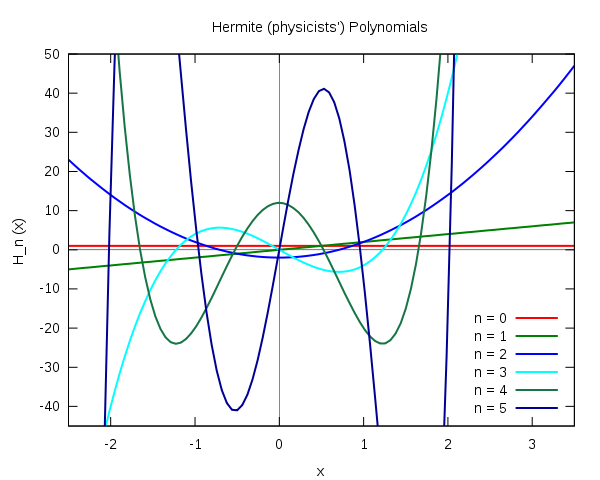
\includegraphics[width=8cm]{images/Hermite_polynomial_matlab_pic.png}
                \caption{Hermite多项式MATLAB图像}
                \label{fig:Hermite多项式MATLAB图像}
                \end{figure}
                % \textcolor[rgb]{1 0 0}{todo:matlab图片:Hermite多项式MATLAB图像}
                \par
                Hermite多项式的正交性
                \begin{align*}
                    \int_{-\infty}^{\infty} e^{-x^2} H_n(x)H_m(x) \mathrm{d}x  = 2^nn!\sqrt{\pi} \delta_{mn}
                \end{align*}
                即$H_n(x)$在$[-\infty,\infty]$上带权$\rho(x) = e^{-x^2}$正交。

                \paragraph{Laguerre多项式}
                Lagurre是下面方程的解
                \begin{align*}
                    xy'' + (1-x)y' +ny = 0
                \end{align*}
                上述方程的广义形式为
                \begin{align*}
                    xy'' + (\alpha +1-x)y' +ny = 0
                \end{align*}
                \par
                Lagurre的表达式为
                \begin{align}
                    \label{eq:Laguerre多项式一般形式}
                    L_n(x) = \sum_{k = 0}^n \binom{n}{k}\frac{(-1)^k}{k!}x^k
                \end{align}
                广义表达式为
                \begin{align*}
                    L_n^{\alpha}(x) = \sum_{k = 0}^n (-1)^k\binom{n+\alpha}{n-k}\frac{x^k}{k!}
                \end{align*}
                \par
                Lagurre的递推公式为
                \begin{align*}
                    &L_0(x) = 1\\
                    &L_1(x) = -x +1\\
                    &L_2(x) = \frac{1}{2} (x^2 - 4x +2)\\
                    &L_3(x) = \frac{1}{6} (-x^3+9x^2 - 18x + 6)\\
                    &L_4(x) = \frac{1}{24}(x^4 -16x^3 +72x^2 -96x +24)\\
                    &\vdots\\
                    &L_{n+1}(x) = \frac{(2n+1 -x)L_n(x) - nL_{n - 1}(x)}{n+1}
                \end{align*}
                广义形式的递推公式为
                \begin{align*}
                    L_n^\alpha (x) = \frac{\alpha + 1-x}{n}L_{n-1}^{\alpha+1} (x) - \frac{x}{n}L_{n-2}^{\alpha+2} (x)
                \end{align*}
                Lagurre的正交性为
                \begin{align*}
                    \int_0^{\infty} x^\alpha e^{-x}L_n^\alpha (x)L_m^\alpha (x) \mathrm{d}x = \frac{\Gamma(n+\alpha+1)}{n!}\delta_{mn}
                \end{align*}

            \subsubsection{非周期边值问题的谱方法}
                \label{subsubsec:非周期边值问题的谱方法}
                \par
                上面介绍了一些正交多项式,下面,我们以Legendre多项式为基组,来求解如下泊松方程
                \begin{align*}
                    \left\{
                        \begin{aligned}
                        &Lu:=\triangle u = f(x,y)\quad (x,y)\in \Omega \\
                        &u(\pm 1, y) = u(x,\pm1) = u\bigl|_{\partial \Omega} = 0 \quad (x,y)\in \partial \Omega
                        \end{aligned}
                    \right.
                \end{align*}
                其中:$\Omega = \{(x,y)|0 \leqslant x,y \leqslant 1\}$。
                \par
                上述问题的G变分问题为:求$u(x,y) \in U$,使得$\forall v(x,y) \in U$,$v(\pm 1, y) = v(x,\pm1) = 0$,有
                \begin{align*}
                    a(u,v) = (f,v)
                \end{align*}
                我们取$U$的有限维空间$U_n = \{u_n(x,y)|\text {特征}\}$为搜索空间,其基组为$\{\varphi_i(x,y)\}$。这里,我们用Legendre多项式$L_n(x),L_m(y)$作为基函数,则基组为$\{L_i(x),L_j(y)\}_{i,j = 0}^n$,于是,$u_n(x,y)$可以用基组表示为
                \begin{align}
                    \label{u的基组形似}
                    u_n(x,y) = \sum_{k = 0}^n c_k \varphi_k(x,y) = \sum_{i = 0}^n\sum_{j = 0}^n a_{ij} L_i(x)L_j(y)
                \end{align}
                注意:$L_i(x),L_j(y)$不必满足边界条件,这点与Galerkin谱方法不同。
                \par
                同理,我们可以用基组表示出$v(x,y)$的估计$v_n(x,y)$
                \begin{align}
                    \label{v的基组形似}
                    v_n(x,y) = \sum_{k = 0}^n c_k \varphi_k(x,y) = \sum_{i = 0}^n\sum_{j = 0}^n b_{ij} L_i(x)L_j(y)
                \end{align}
                由于$v_n(x,y)$具有任意性,那么,不妨令
                \[
                v_{ij} = \varphi_{ij}(x,y) = p_i(x)p_j(y) = \sqrt{\frac{2i+1}{2}}L_i(x)\sqrt{\frac{2j+1}{2}}L_j(x)
                \]
                $\varphi_{ij}(x,y)$可以取遍所有基组($i,j = 0,1,\dots,n -1$),并且注意,只有当$i = j$时,$\varphi_{ij}$才有值,否则为$0$。我们记边界条件为
                \begin{align*}
                    \left\{
                    \begin{aligned}
                        &B_1(u) = u(x,-1)\\
                        &B_2(u) = u(x,1)\\
                        &B_3(u) = u(-1,y)\\
                        &B_4(u) = u(1,y)
                    \end{aligned}
                    \right.
                \end{align*}
                那么,$a(u,v) = (f,v)$可以表示为
                \begin{align*}
                            &a(u,v) = (f,v) \quad \forall v \in U\\
                \implies {} &a(u_n,v_{ij}) = (f,v_{ij}) \quad \forall v_{ij} \in U_n\\
                \implies {} &\iint\limits_{\Omega} \left( \frac{\partial ^2 u_n}{\partial x^2} + \frac{\partial ^2 u_n}{\partial y^2} \right) \varphi_{ij}(x,y) \mathrm{d}x\mathrm{d}y = \iint\limits_{\Omega}f(x,y) \varphi_{ij}(x,y) \mathrm{d}x\mathrm{d}y
                \end{align*}
                \par
                上述方程中共有$n+1$个参数$a_{ij}$,所以我们要构建方程组。当$i,j = 0,1,\dots,n - 1$时,可形成如下方程组
                \begin{align*}
                    \left\{
                        \begin{aligned}
                        &a(u_n,v_{ij}) = (f,v_{ij})\quad i,j = 0,1,\dots,n - 1 \\
                        &\int _{-1}^1 B_1(u_n) p_i(x) \mathrm{d}x =0 \quad i = 0,1,\dots,n\\
                        &\int _{-1}^1 B_2(u_n) p_i(x) \mathrm{d}x = 0\quad i = 0,1,\dots,n\\
                        &\int _{-1}^1 B_3(u_n) p_j(x) \mathrm{d}y = 0\quad j = 0,1,\dots,n\\
                        &\int _{-1}^1 B_4(u_n) p_j(x) \mathrm{d}y =0 \quad j = 0,1,\dots,n
                        \end{aligned}
                    \right.
                \end{align*}
                利用Legendre多项式$L_n(x)$的正交性,解上述方程可以得到解$\{a_{ij}\}_{i,j = 0}^n$。

\section{符号和函数空间注记}
    \subsection{符号注记}
        PDE篇常用的数学符号解释
        \par
        $\mathbb{N}$表示整数集合
        \par
        $R$表示实数集合
        \par
        $R^n$表示$n$维欧式空间
        \par
        $\Omega$表示$R^n$的子集(域),是连同开集
        \par
        $\partial \Omega$表示$\Omega$的边界
        \par
        $\triangle$表示Laplace算子,$\triangle u = \sum_{i = 1}^n\frac{\partial^2 u}{\partial x_i^2}$
        \par
        $\nabla$表示梯度算子(哈密顿算子)
        \par
        $C_0^m(\Omega)$表示$\Omega$上有紧支集的函数集合
        \par
        $C_0^{\infty}(\Omega)$表示$\Omega$上有紧支集的无穷次可微函数的集合
        \par
        $C^{\infty}(\Omega)$表示$\Omega$上无穷次可微函数的集合
        \par
        $L_{loc}^1 (\Omega)$表示$\Omega$上局部可积函数集,对任意有界可测集$E \subset \Omega$,$f$在$E$上Lebesgue可积
        \par
        $L^p(\Omega)$表示$\Omega$上$p$次Lebesgue可积函数集
        \par
        $U$表示函数$u$的求解空间,是Sobolev空间
        \par
        $U_n$表示无穷维空间$U$的$n$维有穷维空间
        \par
        $u_n$表示函数$u$的估计,$u_n \in U_n$
        \par
        $H_E^1$是函数集$H_n \equiv U_n$的子集(子空间)
    \subsection{函数空间注记}
        \paragraph{距离空间}
        $E$是一个非空集合(不妨设为函数集合),如果$\forall x,y \in E$,$\exists d(x,y) \in R$,$d$满足:1、非负2、对称3、三角不等式,则称$d$为$x,y$的距离,$E$为距离空间。
        \paragraph{线性空间}
        $H$是一个非空集合,如果$H$中的元素$x,y$对加法和数量乘法封闭,则称$H$为线性空间。
        \paragraph{线性赋范空间}
        $H$是一个线性空间,$H$中的每一元素$x$,按某一规则对应一非负实数$||x||$,且满足\\
        1、$||x|| \geqslant 0$。如果$||x|| = 0$,则$x = 0$,这里的$0$是空间$H$的$0$元素。\\
        2、$||\alpha x|| = |\alpha|\ ||x||$, $\forall \alpha \in R,\forall x \in H$。\\
        3、$||x +y|| \leqslant ||x||+||y||$,$\forall x,y \in H$。\\
        则称$H$为赋范线性空间(线性并且范数存在,线性赋范),称$||x||$为$x$的范数。
        \paragraph{Banach空间}
        设$H$是一个距离空间,$M,E \subset H$。如果对于$H$中的任意元素$x$的任意邻域均含有$M$中的点,则称$M$在$E$中稠密;如果$H$中的任一基本序列都有机选,且极限点属于$H$,则称$H$为完备空间。完备的线性赋范空间为Banach空间。
        \paragraph{$L^p(\Omega)$空间}
        记$\Omega$上Lebesgue可测且$p$次可积$\int_{\Omega} |f(x)|^p \mathrm{d}x < +\infty$的函数全体为$L^p(\Omega)$。
        其中:$1<p<\infty$。
        \par
        若令
        \[
            ||f||_{L^p(\Omega)} = \left( \int_{\Omega} |f(x)|^p \mathrm{d}x\right)^{\frac{1}{p}}
        \]
        为范数,则$L^p(\Omega) = \{f|\ ||f||_{L^p(\Omega)} < \infty\}$。
        \par
        $L^p(\Omega)$是一个Banch空间,$L^p(\Omega)$空间中有下列重要不等式\\
        1、Minibowski不等式。如果$1 \leqslant p \leqslant +\infty$,则$\forall f,g \in L^p(\Omega)$,有
        \[
            ||f +g||_{L^p(\Omega)} \leqslant ||f||+||g||
        \]
        2、Holder不等式。如果$1 \leqslant p,q \leqslant +\infty$,$\frac{1}{p} + \frac{1}{q} = 1$,则$\forall f \in L^p(\Omega),g\in L^q(\Omega)$,有$fg \in \in L^1(\Omega)$且
        \[
            ||f g||_{L^1(\Omega)} \leqslant ||f||_{L^p(\Omega)}||g||_{L^q(\Omega)}
        \]
        3、Schwarz不等式。如果$p = q = 2$,则$\forall f,g \in L^2(\Omega)$,有$fg \in L^1(\Omega)$且
        \[
            ||f g||_{L^1(\Omega)} \leqslant ||f||_{L^2(\Omega)}||g||_{L^2(\Omega)}
        \]
        \paragraph{内积空间}
        设$H$为线性空间,若$\forall x,y \in H$,$\exists \bigl<x,y\bigr>\in R$与之对应,且满足
        1、$\bigl<x,y\bigr> \geqslant 0$,$\forall x,y \in H$\\
        2、$\bigl<x+y,z\bigr> = \bigl<x,z\bigr> + \bigl<y,z\bigr>$,$\forall x,y,z \in H$\\
        3、$\bigl<\alpha x,y\bigr> = \alpha \bigl<x,y\bigr> $,$ \forall \alpha \in R,\forall x,y \in H$\\
        4、$\bigl<x,y\bigr> = \bigl<y,x\bigr> $,$\forall x,y \in H$\\
        则称$<x,y>$为$x,y$的内积,$H$为内积空间。在实内积空间中,有
        \begin{align*}
            &||x|| = \sqrt{\bigl<x,y\bigr>}\\
            &\theta = \arccos \frac{\bigl<x,y\bigr>}{||x||\ ||y||}
        \end{align*}
        \paragraph{Hilbert空间}
        完备的内积空间为Hilbert空间,Hilbert是Banch空间。西伯尔特空间为基于任意正交系上的多项式表示的傅里叶级数和傅里叶变换提供了有效的表达方式。
        \paragraph{广义导数}
        设$u \in L_{loc}^1 (\Omega)$(即$u$在$\Omega$上局部可积),而且$\exists v\in L_{loc}^1 (\Omega)$,有
        \begin{align*}
            \int_{\Omega} v \varphi \mathrm{d}x = -\int_{\Omega}u \frac{\partial \varphi}{\partial x_i} \mathrm{d}x \quad \forall \varphi \in C_0^{\infty}(\Omega)
        \end{align*}
        其中:$x_i$为自变量$x$的分量,$i = 1,2,\dots,n$。称$v$是$u$对$x_i$的一阶广义导数,记为$v = \frac{\partial \varphi}{\partial x_i}$。
        \par
        如果$u \in L_{loc}^1 (\Omega)$,$\exists v\in L_{loc}^1 (\Omega)$ ,使得
        \begin{align*}
            \int_{\Omega} v \varphi \mathrm{d}x = (-1)^{|\alpha|}\int_{\Omega}u {\partial^{\alpha} \varphi}\mathrm{d}x \quad \forall \varphi \in C_0^{\infty}(\Omega)
        \end{align*}
        则称$v$是$u$的$\alpha$阶广义导数,记为$v= \partial^{\alpha} u$。

        \paragraph{Sobolev空间}
        设$m$为非负正数,$1 \leqslant p \leqslant +\infty$,记
        \begin{align*}
            S^{mp}(\Omega) = \{u\in L^p(\Omega) |  \partial^{\alpha} u \in L^p(\Omega) ,|\alpha| \leq m \}
        \end{align*}
        并且赋与范数
        \begin{align*}
            &||u||_{m,p} = \left( \sum_{|\alpha| \leq m } ||\partial^{\alpha} u ||_{L^p(\Omega)}^p \right)^{\frac{1}{p}}\\
            &||u||_{m,\infty} = \max_{|\alpha| \leq m } ||\partial^{\alpha} u ||_{0,\infty}
        \end{align*}
        则称线性赋范空间$S^{mp}(\Omega)$为Sobolev空间。

\section{MATLAB解偏微分方程}
    \par
    下面偏微分方程的写法我们用Laplace算子和哈密顿算子表示。Laplace算子和哈密顿算子在前面介绍过了,这里不再介绍。我们可以将二维泊松方程写为如下三种形式
    \begin{align*}
        &- \left( \frac{\partial ^u}{\partial x^2} +\frac{\partial ^u}{\partial y^2} \right) = f(x,y)\\
        &- \triangle u = f(x,y)\\
        &- \nabla\cdot \nabla u = f(x,y)
    \end{align*}
    \par
    给出方程的表达式之后,我们需要继续讨论变量的范围以及方程的边界条件。我们仍然沿用前面的符号,用$\Omega$表示$R^n$上的有界区域,用$\partial \Omega$表示$\Omega$的边界,有了这些之后,我们就可以求解具体的偏微分方程了。下面,将展示如何运用MATLAB来求解PDE问题。值得一提的是,由于二维图像更容易绘制,所以我们往往在$\Omega \in R^2$上求解函数$u(x,y)$,将一维情况$u(x)$扩展到二维,将三维情况$u(x,y,t)$压缩到二维,下面的示例都是求解$u(x,y)$或者$u(x,t)$的情形。
    关于PDE的数值方法,前面我们主要介绍了有限差分法、有限元方法和谱方法,下面,我们给出其MATLAB示例。

    \subsection{有限元解法}
        \par
        MATLAB自带的工具箱PDEtoolbox是运用有限元方法求解偏微分问题的,它们是使用最广泛的方法和工具箱。我们先来看一下PDEtoolbox能求解的方程类型和边界条件。
        \paragraph{方程类型}PDEtoolbox能求解的方程类型有如下几种:
        \par
        1.椭圆型方程
        \[
            - \nabla (c\nabla u) + au = f, \quad \Omega
        \]
        其中:$\Omega \in R^2$,$c,a,f$为$\Omega$上的实函数,$u$为$\Omega$上的待求函数。
        \par
        2.抛物型方程
        \[
            d \frac{\partial u}{\partial t} - \nabla(c\nabla u)+au = f, \quad \Omega
        \]
        \par
        3.双曲型方程
        \[
            d \frac{\partial^2 u}{\partial t^2} - \nabla(c\nabla u)+au = f, \quad \Omega
        \]
        \par
        4.特征方程
        \[
            -\nabla (c\nabla u)+au = \lambda du, \quad \Omega
        \]
        其中:$\Omega \in R^2$,$c,a,f$为标量复函数形式系数,可以是时间$t$的函数,$\lambda$为待求本征值,$u$为$\Omega$上的待求函数。
        \par
        5.非线性椭圆方程
        \[
            -\nabla (c(u) \nabla u) + a(u)u = f(u), \quad \Omega
        \]
        其中:$c,a,f$可以是$u$的函数。
        \par
        6.偏微分方程组
        \begin{align*}
            \left\{
            \begin{aligned}
            -\nabla(c_{11}\nabla {u_1}) - \nabla(c_{12}\nabla {u_2}) + a_{11}u_1 +a_{12} u_2 = f_1\\
            -\nabla(c_{21}\nabla {u_1}) - \nabla(c_{22}\nabla {u_2}) + a_{21}u_1 +a_{22} u_2 = f_1
            \end{aligned}
            \right.
        \end{align*}
        \paragraph{边值条件类型}PDEtoolbox能求解的方程边值条件有如下几种类型:
        \par
        1. Dirichlet条件
        \[
            hu = r,\quad \partial \Omega
        \]
        \par
        2. Neumann条件
        \[
            \mathbf{n} (c\nabla u)+qu = g,\quad \partial \Omega
        \]
        其中:$\mathbf{n}$为$\partial \Omega$上的单位外法向矢量;$g,r,q,h,c$为$\partial \Omega$上的函数。
        \par
        对于特征值问题,要求$g = r =0$;对于非线性问题,$g,q,r,h,c$可以是$u$的函数;对于抛物型和双曲型方程,$g,r,h,c,q$可以是时间$t$的函数;对于方程组而言,Dirichlet条件为
        \begin{align*}
            h_{11} u_1 +h_{12}u_2 = r_1\\
            h_{21} u_1 +h_{22}u_2 = r_2
        \end{align*}
        而Neumann条件为
        \begin{align*}
            \mathbf{n} (c_{11} \nabla u_1) + \mathbf{n} (c_{12} \nabla u_2) + q_{11}u_1 + q_{12} u_2 = g_1 \\
            \mathbf{n} (c_{21} \nabla u_1) + \mathbf{n} (c_{22} \nabla u_2) + q_{21}u_1 + q_{22} u_2 = g_2
        \end{align*}
        混合边界条件为
        \begin{align*}
            &h_{11}u_1 +h_{12}u_2 = r\\
            &\mathbf{n} (c_{11} \nabla u_1) + \mathbf{n} (c_{12} \nabla u_2) + q_{11}u_1 + q_{12} u_2 = g_1 + h_{11}\mu\\
            &\mathbf{n} (c_{21} \nabla u_1) + \mathbf{n} (c_{22} \nabla u_2) + q_{11}u_1 + q_{12} u_2 = g_1 + h_{12}\mu
        \end{align*}
        其中:$\mu$的计算要使得Dirichlet条件满足。
        \paragraph{有限元步骤}下面,我们用椭圆型方程快速概述一下有限元法的步骤。考虑基本的椭圆方程
        \begin{align*}
            \left\{
            \begin{aligned}
            &-\nabla (c\nabla u)+au = f & \Omega\\
            &hu = r & \partial \Omega \\
            &\mathbf{n}(c\nabla u) +qu = g & \partial \Omega
            \end{aligned}
            \right.
        \end{align*}
        \par
        \ding{172}上述问题的G变分问题为:求$u \in U$,使得$\forall v \in U$,有
        \begin{align*}
            \int _{\Omega} [- (\nabla(c\nabla u)v + auv)] \mathrm{d}x\mathrm{d}y = \int _{\Omega}fv\mathrm{d}x\mathrm{d}y
        \end{align*}
        对上面的G变分问题使用Green公式,有
        \begin{align*}
            \int _{\Omega} [ (c\nabla u)\nabla v + auv] \mathrm{d}x\mathrm{d}y - \int _{\Omega} (-qu+g)v\mathrm{d}s
             = \int _{\Omega}fv\mathrm{d}x\mathrm{d}y
        \end{align*}
        \par
        \ding{173}设$u(x,y),v(x,y)$可以近似表示为分片多项式的形式。$\{\varphi_i(x,y)\}$为空间$U_n$的基组,有
        \begin{align*}
            u_n(x,y) = \sum_{i = 1}^n \varphi_i c_i \\
            v_n(x,y) = \sum_{i = 1}^n \varphi_i d_i
        \end{align*}
        其中:$c_i$为待求系数。
        \par
        \ding{174}区域$\Omega$的划分。用三角形元将$\Omega$划分为$N_e$个单元,$N_p$个顶点。一般而言,在使用三角形元时,要注意:
        1.单元顶点不能是相邻单元边上的内点;
        2.避免出现大的钝角和大的边;
        3.在$u(x,y)$的梯度变化较剧烈的地方,网格要加密;
        4.单元编号可以任意,但节点编号应尽量使所有两个相邻节点编号只差的绝对值中最大值越小越好
        \begin{align*}
        &\min\max_{|i-j| = 1}|i,j|\\
        &s.t.
            \left\{
            \begin{aligned}
            i = 1,2,\dots,N_p\\
            j = 1,2,\dots,N_p
            \end{aligned}
            \right.
        \end{align*}
        \par
        \ding{175}单元$e$上的多项式。在单元$e$上假设$u_e(x,y)$为分片一次多项式,即
        \[
            u_e(x,y) = ax+by+c
        \]
        设在$e$的各定点$(i,j,k)$处的函数值为$u_i,u_j,,u_k$,记$u_e = [u_i,u_j,u_k]^\mathrm{T}$,可以计算
        \[
            u_e(x,y) = \mathbf{N} u_e
        \]
        及梯度
        \[
            \nabla u_e(x,y) = \mathbf{B}u_e
        \]
        \par
        \ding{176}计算单元刚度矩阵,单元载荷向量。
        \begin{align*}
            \sum_{k = 1}^{N_e} \iint\limits_{e_k} [(c\nabla u_e)\nabla v_e+au_ev_e]\mathrm{d}e - \int_{\partial \Omega}(-q u_e+g)v_e \mathrm{d}s = \sum_{k = 1}^{N_e}\iint\limits_{e_k} fv_e \mathrm{d}e
        \end{align*}
        这里,三角单元的梯度$\nabla u_e$和面积$S_e = \iint\limits_{e_k} \cdot \mathrm{d}e$是通过MATLAB的pdetrg实现的,得到单元刚度矩阵$K_e$,和单元载荷向量$F_e$。
        \par
        \ding{177}总刚度矩阵和总载荷向量。首先,对$F_e,K_e$进行扩充,MATLAB通过eassemple函数实现的;然后,再求解总刚度矩阵$K$和总载荷向量$F$,MATLAB通过assempde函数实现。\\
        \ding{178}对于Neumann条件,$\partial \Omega$上不需要满足任何约束条件,由此可以求得
        \[
            KU = F
        \]

    \subsection{MATLAB应用实例}
        \subsubsection{示例1:单位圆上的泊松问题(椭圆型)}
            \par
            \begin{align*}
                \left\{
                \begin{aligned}
                &-\triangle u = 1\\
                &\Omega = \{(x,y)|x^2+y^2<1\}\\
                &u\bigl|_{\partial \Omega} = 0
                \end{aligned}
                \right.
            \end{align*}
            此问题的精确解为
            \begin{align*}
                u(x,y) = \frac{1-x^2-y^2}{4}
            \end{align*}
            此问题的求解程序如下
            \begin{lstlisting}[language = Matlab]
            %%%%%%%%%%%%%%% 示例1:单位圆上的Poisson方程 %%%%%%%%%%%%%%%%
            %% 旧方法
            %------------------------------------------------------------
            %一般方程形式为: -div(c*grad(u)) + a*u = f,
            %我们要解的方程为:c = 1; a = 0; f = 1;
            %------------------------------------------------------------
            clc, clear
            g = @circleg; b = @circleb1;
            c = 1; a = 0; f = 1;
            [p, e, t] = initmesh(g, 'hmax', 1); %初始化网格。x = p(1,:);y = p(2,:)
            % pdemesh(p, e, t);%绘制网格,p的第一行和第二行为x,y坐标,e是边界矩阵
            error = [];
            err = 1;
            while err > 0.001;
                [p, e, t] = refinemesh(g, p, e, t); %加密网格
                u = assempde(b, p, e, t, c, a, f); %求解u。组成偏微分方程刚度矩阵及其右边
                exact = (1-p(1,:).^2 - p(2,:).^2)'/4; %精确解
                err = norm(u - exact, 'inf'); %计算误差
                error = [error, err];
            end
            figure
            pdemesh(p, e, t);%绘制网格
            figure
            pdesurf(p, t, u);%绘制解的曲面
            figure
            pdesurf(p, t, u - exact);%绘制误差图
            %% 新方法
            %------------------------------------------------------------
            %一般方程形式为:m*Utt + d*Ut - div(c*grad(u)) + a*u = f,
            %我们要解的方程为:- div(c*grad(u)) = 1.
            %------------------------------------------------------------
            clc, clear
            % 确定方程(模型系数及边界形状)
            m = 0; d = 0; c = 1; a = 0; f = 1;
            g = @circleg;%边界形状g,@lshapeg
            figure
            pdegplot(g,'EdgeLabels','on');%查看边界形状g,并打开边界标号
            axis equal
            % 创建一个PDE模型--pdemodel
            numberOfPDE = 1;%偏微分方程(组)的个数
            pdemodel = createpde(numberOfPDE);%返回一个n个方程的偏微分方程模型容器。
            geometryFromEdges(pdemodel, g);%创建一个几何实体,oumiga
            specifyCoefficients(pdemodel,'m',m,'d',d,'c',c,'a',a,'f',f);%指定模型的系数
            applyBoundaryCondition(pdemodel,'Edge',(1:4),'u',0);%设置pdem的边界条件
            hmax = 1;
            generateMesh(pdemodel,'Hmax',hmax);%形成单元e
            %
            figure
            pdemesh(pdemodel);
            axis equal
            er = Inf;
            while er > 0.001
                hmax = hmax/2;
                generateMesh(pdemodel,'Hmax',hmax);
                result = solvepde(pdemodel); %解pdem
                msh = pdemodel.Mesh;% 第一行为x坐标,第二行为y坐标
                u = result.NodalSolution;
                exact = (1 - msh.Nodes(1,:).^2 - msh.Nodes(2,:).^2)'/4; %解析解
                er = norm(u-exact,'inf');
                fprintf('Error: %e. Number of nodes: %d\n',er,size(msh.Nodes,2));
            end
            figure
            pdemesh(pdemodel);
            axis equal
            figure
            pdeplot(pdemodel,'XYData',u,'ZData',u,'ColorBar','off')
            \end{lstlisting}
            新旧方法求解结果如图(\ref{单位圆上的泊松问题})所示
            \begin{figure}[H]
                \centering
                \begin{subfigure}[b]{0.4\textwidth}
                    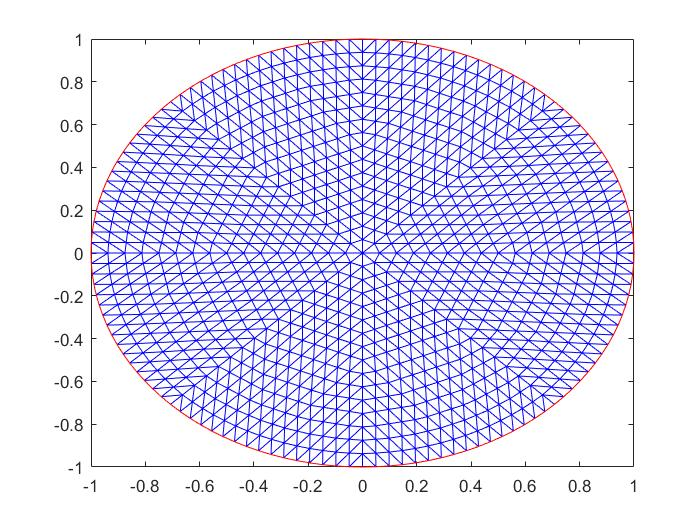
\includegraphics[width=\textwidth]{images/PDE_example_oldmethod_wangge.jpg}
                    % \caption{旧方法}
                    % \label{}
                \end{subfigure}
                \begin{subfigure}[b]{0.4\textwidth}
                    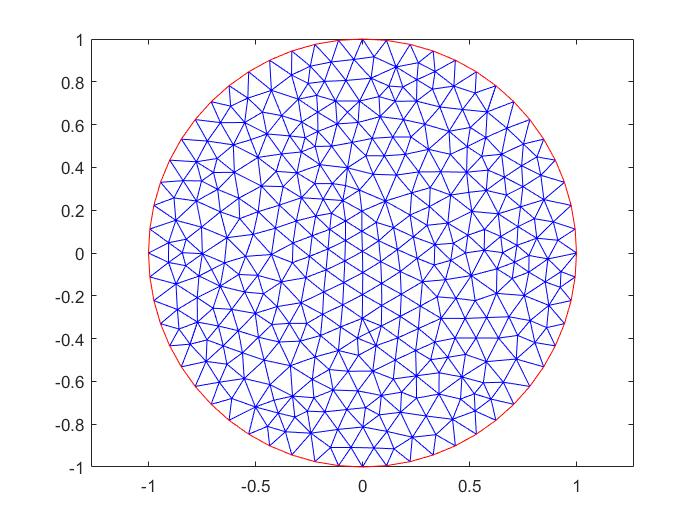
\includegraphics[width=\textwidth]{images/PDE_example_newmethod_wangge.jpg}
                    % \caption{新方法}
                    % \label{}
                \end{subfigure}
                \begin{subfigure}[b]{0.4\textwidth}
                    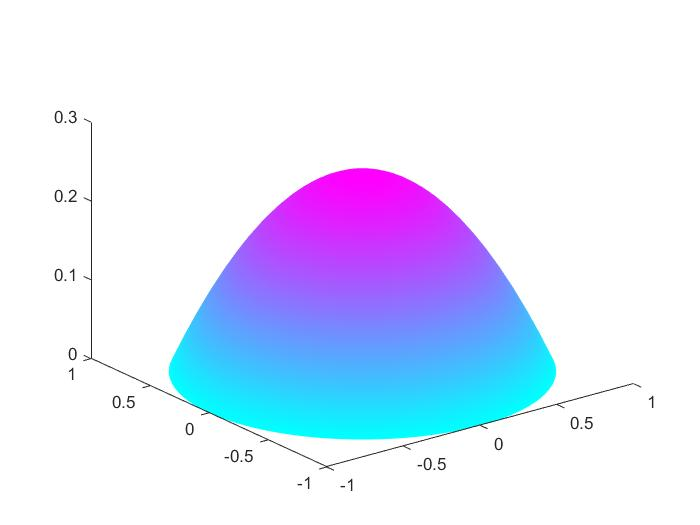
\includegraphics[width=\textwidth]{images/PDE_example_oldmethod_jieguo.jpg}
                    \caption{旧方法}
                    % \label{}
                \end{subfigure}
                \begin{subfigure}[b]{0.4\textwidth}
                    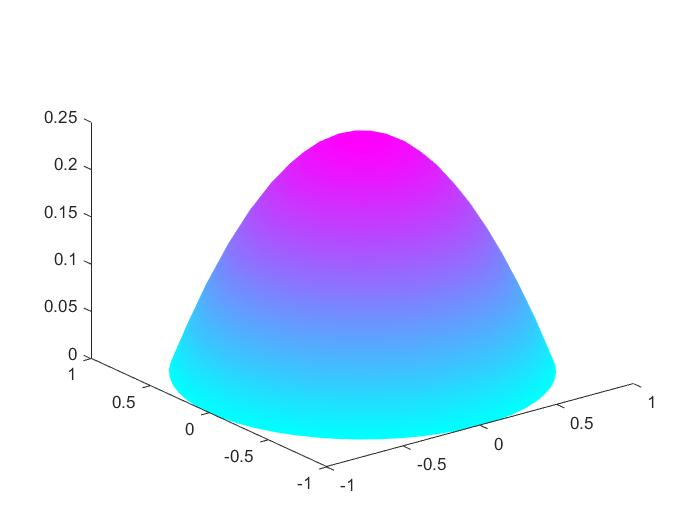
\includegraphics[width=\textwidth]{images/PDE_example_newmethod_jieguo.jpg}
                    \caption{新方法}
                    % \label{}
                \end{subfigure}
                \caption{单位圆上的泊松问题}
                \label{单位圆上的泊松问题}
            \end{figure}

        \subsubsection{示例2:单位正方形上的波动方程(双曲型)}
            \par
            \begin{align*}
                \left\{
                \begin{aligned}
                    & \frac{\partial^2 u}{\partial t^2} -\nabla\cdot\nabla u = 0\\
                    &\Omega = \{(x,y)|0 \leqslant x,y \leqslant 1\}\\
                    &\text{初值条件:}\\
                    &u(x,0) = \arctan\left(\cos\left(\frac{\pi x}{2}\right)\right)\\
                    &\frac{\partial u}{\partial t} \Bigl|_{t = 0} = 3\sin(\pi x) e^{\sin \left( \frac{\pi y}{2}\right)}\\
                    &\text{边界条件:}\\
                    &u\bigl|_{x = \pm 1} = 0\quad \text{2,4边为Dirichlet条件}\\
                    &\frac{\partial u}{\partial \mathbf{n}} \Bigl|_{y = \pm 1}  = 0 \quad\text{1,3边为Neumann条件}
                \end{aligned}
                \right.
            \end{align*}
            求解程序如下
            \begin{lstlisting}[language = Matlab]
            %%%%%%%%%%%%%%%%%%%%%%%%%  示例2:波动方程 %%%%%%%%%%%%%%%%%%%
            %------------------------------------------------------------
            %波动方程的一般形式为:d*Utt - div(c*giadU) + a*U = f
            %我们要解决的二维波动方程为:Utt - div(c*giadU) = 0;
            %------------------------------------------------------------
            %% 旧方法
            clc, clear
            c = 1; a = 0; f = 0; d = 1;
            g = @squareg;%边界区域
            b = @squareb3;
            [p, e, t] = initmesh(g);%初始化网格
            x = p(1, :)';
            y = p(2, :)';
            u0 = atan(cos(pi/2*x));%初始条件
            ut0 = 3*sin(pi*x).*exp(sin(pi/2*y));%初始条件
            n = 31;
            tlist = linspace(0, 5, n);%离散时间
            uu = hyperbolic(u0, ut0, tlist, b, p, e, t, c, a, f, d);%求解双曲线型PDE方程,uu是一个31列的矩阵,每个时间t为一列
            delta = -1:0.1:1;
            [uxy, tn, a2, a3] = tri2grid(p, t, uu(:, 1), delta, delta);%将三角形网格转化为矩形网格
            gp = [tn;a2;a3];
            umax = max(max(uu));
            umin = min(min(uu));
            newplot
            M = moviein(n);
            for i = 1:n
                pdeplot(p, e, t, 'xydata', uu(:, i), 'zdata', uu(:, i), ...
                    'mesh', 'off', 'xygrid', 'on', 'gridparam', gp,...
                    'colorbar', 'off', 'zstyle', 'continuous');
                axis([-1, 1, -1, 1, umin, umax]);
                caxis([umin, umax]);
                M(:, i) = getframe;
            end
            movie(M, 10);
            %% 新方法
            %-----------------------------------------------------------------------
            %方程的一般形式为:m*Utt + d*Ut - div(c*giadU) + a*U = f
            %我们要解决的二维波动方程为:Utt - div(c*giadU) = 0;
            %-----------------------------------------------------------------------
            clc, clear
            % 1、确定方程(模型系数,边界形状)
            m = 1; d = 0; c = 1; a = 0; f = 0;
            g = @squareg;
            numberOfPDE = 1;
            model = createpde(numberOfPDE);
            geometryFromEdges(model, g);
            % pdegplot(model,'edgeLabels','on');
            % ylim([-1.1 1.1]);
            % axis equal, title 'Geometry With Edge Labels Displayed', xlabel x, ylabel y
            %2、确定边界条件
            specifyCoefficients(model,'m',m,'d',d,'c',c,'a',a,'f',f);
            applyBoundaryCondition(model, 'Edge',[2,4], 'u', 0);%dirichlet边界条件
            applyBoundaryCondition(model, 'Edge',[1 3], 'g', 0);%neumann边界条件
            %3、形成最终模型
            generateMesh(model);%形成单元e
            u0 = @(location) atan(cos(pi/2*location.x));%初始条件
            ut0 = @(location) 3*sin(pi*location.x).*exp(sin(pi/2*location.y));%初始条件
            setInitialConditions(model, u0, ut0);%设置初始条件
            %4、求解模型
            n = 31;
            tlist = linspace(0,5,n);
            model.SolverOptions.ReportStatistics = 'on';
            result = solvepde(model, tlist);%解PDE模型
            u = result.NodalSolution;%u是一个31列的矩阵,每个时间t为一列
            figure
            umax = max(max(u));
            umin = min(min(u));
            for i = 1:n
                pdeplot(model,'xydata',u(:,i),'zdata',u(:,i),'zstyle','continuous',...
                              'mesh','off','xygrid','on','colorbar','off');
                axis([-1 1 -1 1 umin umax]);
                caxis([umin umax]);
                xlabel x, ylabel y, zlabel u
                M(i) = getframe;
            end
            movie(M, 1);
            \end{lstlisting}
            用新方法求解上述问题,最终停止时的结果如图(\ref{单位正方形上的波动方程})所示
            \begin{figure}[H]
            \centering
            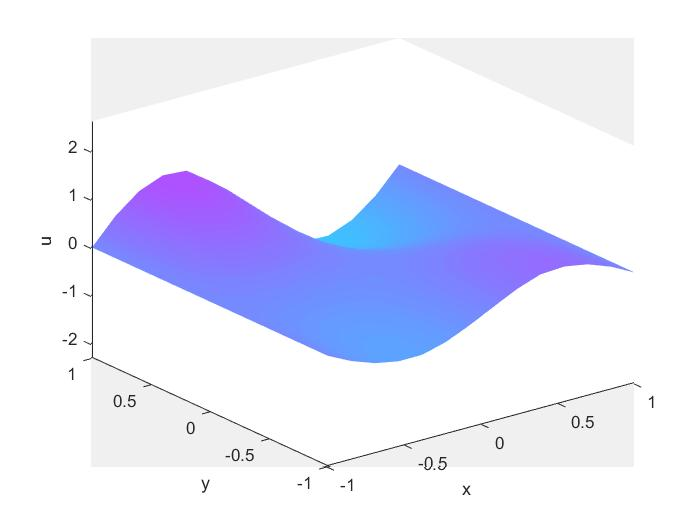
\includegraphics[width = 8cm]{images/PDE_example2_newmethod_jieguo.jpg}
            \caption{单位正方形上的波动方程}
            \label{单位正方形上的波动方程}
            \end{figure}
        \subsubsection{示例3:薄板中的非线性传热(抛物型方程)}
            \par
            一般形式的热传导方程如下
            \begin{align*}
                \rho c \frac{\partial T}{\partial t} - \nabla(k \nabla T) = Q + h(T_Q - T)
            \end{align*}
            其中:$\rho$为密度,$c$为比热容,$k$为导热系数,$Q$为热源,$h$为对流热的传输系数,$T_Q$为环境温度,$h(T_Q - T)$表示从环境向区域内部传输的热量。
            \par
            如果仅考虑稳态情况$\frac{\partial T}{\partial t} = 0$,有
            \begin{align*}
            - \nabla (k\nabla T) = Q +h(T_1- T)
            \end{align*}
            令
            \[
            Q_c = h_c(T - T_a)
            \]
            其中:$T_a$是环境温度,$h_c$是热对流系数。
            \par
            从单位面积辐射的热转移量为
            \begin{align*}
                Q_r = \epsilon \sigma (T^4 - T_a^4)
            \end{align*}
            其中:$\epsilon$为薄板发射率,$\sigma$是波尔兹曼常数。
            \begin{align*}
                \rho c t_2\frac{\partial T}{\partial t} - kt_2\nabla^2 T = -2Q_c - 2Q_r
            \end{align*}
            其中:$\rho$为密度,$c$为比热容,$t_2$为薄板厚度。
            \begin{align*}
                \rho c t_2\frac{\partial T}{\partial t} - kt_2\nabla^2 T + 2 h_c T+2\epsilon \sigma T^4 = 2h_cT_a + 2\epsilon \sigma T_a^4
            \end{align*}
            上述问题的求解程序如下
            \begin{lstlisting}[language = Matlab]
            %%%%%%%%%%%%%%% 示例3:金属板的热传导问题 %%%%%%%%%%%%%%%%
            %% 旧方法
            %-------------------------------------------------------------------
            %抛物线方程的一般形式:d*Ut - div(c*gradU) + a*U = f
            %带求解的抛物线方程为:d*Ut - div(c*gradU) = 0
            %-------------------------------------------------------------------
            clc, clear
            % 设置方程系数
            c = 1; a = 0; f = 1; d = 1;
            %设置区域
            R1 = [3;4;-1;1;1;-1;-1;-1;1;1];
            C1 = [1;0;0;0.4];
            C1 = [C1;zeros(length(R1) - length(C1),1)];
            gd = [R1,C1];
            sf = 'R1+C1';
            ns = char('R1','C1')';
            g = decsg(gd,sf,ns);
            %
            numberOfPDE = 1;
            model = createpde(numberOfPDE);%创建一个PDEmodel
            geometryFromEdges(model, g);%创建二维几何
            applyBoundaryCondition(model,'Edge',(1:4),'u',0);%边界条件
            setInitialConditions(model,0);%初始条件,圆(Face2)内为1,圆外为0。
            setInitialConditions(model,1,'Face',2);%初始条件
            msh = generateMesh(model);%有限元划分
            %
            nframes = 20;
            tlist = linspace(0,0.1,nframes);%设置离散时间
            model.SolverOptions.ReportStatistics = 'on';
            u = parabolic(0, tlist, model, c, a, f, d);%用parabolic求解抛物型方程
            %
            figure
            umax = max(max(u));
            umin = min(min(u));
            for j = 1:nframes,
                pdeplot(model,'XYData',u(:,j),'ZData',u(:,j));
                caxis([umin umax]);
                axis([-1 1 -1 1 0 1]);
                M(j) = getframe;
            end
            %% 新方法
            %-------------------------------------------------------------------
            %方程的一般形式:m*Utt + d*Ut - div(c*gradU) + a*U = f
            %带求解的抛物线方程为:d*Ut - div(c*gradU) = 0
            %-------------------------------------------------------------------
            clc, clear
            m = 0; d = 1; c = 1; a = 0; f = 1;
            %
            R1 = [3;4;-1;1;1;-1;-1;-1;1;1];
            C1 = [1;0;0;0.4];
            C1 = [C1;zeros(length(R1) - length(C1),1)];
            gd = [R1,C1];
            sf = 'R1+C1';
            ns = char('R1','C1')';
            g = decsg(gd,sf,ns);
            %
            numberOfPDE = 1;
            model = createpde(numberOfPDE);
            geometryFromEdges(model, g);
            applyBoundaryCondition(model,'Edge',(1:4),'u',0);
            specifyCoefficients(model,'m',m,...
                                     'd',d,...
                                     'c',c,...
                                     'a',a,...
                                     'f',f);
            setInitialConditions(model,0);
            setInitialConditions(model,1,'Face',2);
            msh = generateMesh(model);
            nframes = 20;
            tlist = linspace(0,0.1,nframes);
            model.SolverOptions.ReportStatistics ='on';
            result = solvepde(model,tlist);
            u1 = result.NodalSolution;
            %
            figure
            umax = max(max(u1));
            umin = min(min(u1));
            for j = 1:nframes,
                pdeplot(model,'XYData',u1(:,j),'ZData',u1(:,j));
                caxis([umin umax]);
                axis([-1 1 -1 1 0 1]);
                Mv(j) = getframe;
            end
            \end{lstlisting}
            最终停止时的结果如图(\ref{薄板中的非线性传热})所示
            \begin{figure}[H]
            \centering
            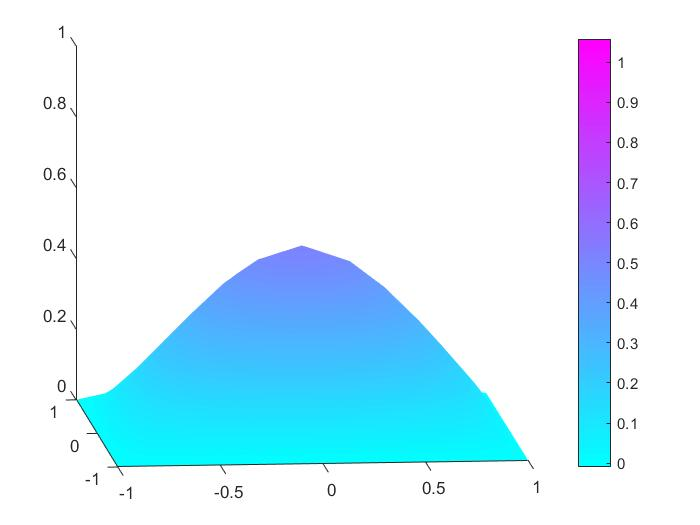
\includegraphics[width = 8cm]{images/PDE_example3_newmethod_jieguo.jpg}
            \caption{薄板中的非线性传热}
            \label{薄板中的非线性传热}
            \end{figure}

        %\subsubsection{示例4:}

    %\subsection{谱分析解法}

% \end{document}
